\Chapter{Closed Form Solutions for Planar ODEs}
\label{Chap:Planar}

\normalsize

In this chapter we describe three different methods to find closed form
solutions to planar constant coefficient systems of linear differential
equations.  In Section~\ref{S:6.1} we begin by discussing those systems of
differential equations that have unique solutions to initial value problems,
and these systems include linear systems.  Then we show how uniqueness to
initial value problems implies that the space of solutions to a constant
coefficient system of $n$ linear differential equations is $n$ dimensional.
Using this observation we present a direct method for solving planar linear
systems in Section~\ref{S:TDM}.  This method extends the discussion of
solutions to systems whose coefficient matrices have distinct real
eigenvalues given in Section~\ref{S:IVPR} to the cases of complex
eigenvalues and equal real eigenvalues.

The matrix exponential is an elementary function that allows us to solve
all initial value problems for constant coefficient linear systems, and
this function is introduced in Section~\ref{S:Matrixexp}.  In
Section~\ref{S:LNFPS} we compute the matrix exponential for several
special, but important, examples.

We compute matrix exponentials in two different ways.  The first approach is
based on changes of coordinates.  The idea is to make the coefficient matrix
of the differential equation as simple as possible; indeed we put the
coefficient matrix in the form of one of the matrices whose exponential is
computed in Section~\ref{S:LNFPS}.  This idea leads to the notion of
{\em similarity\/} of matrices, which is discussed in Section~\ref{S:6.5}, and
leads to the second method for solving planar linear systems. Both the direct
method and the method based on similarity require being able to compute the
eigenvalues {\em and\/} the eigenvectors of the coefficient matrix.

Once these ideas have been introduced and discussed, we use the
Cayley Hamilton theorem to derive a computable formula for all matrix
exponentials of $2\times 2$ matrices.  This formula requires knowing
the eigenvalues of the coefficient matrix --- but not its eigenvectors.
See Section~\ref{S:6.6}.

In the last section of this chapter, Section~\ref{S:SOE}, we consider
solutions to second order equations by reduction to first order systems.


\Section{The Initial Value Problem} \index{initial value problem}
\label{S:6.1}

Recall that a planar autonomous \index{autonomous} system of
ordinary differential equations has the form
\arraystart
\begin{equation}  \label{2dsystem}
\begin{array}{ccl}
\dps \frac{dx}{dt}  & = & f(x,y) \\
\dps \frac{dy}{dt}  & = & g(x,y).
\end{array}
\end{equation}
\arrayfinish
Computer experiments using {\sf pplane5} always appear to find a unique
solution to initial value problems.  More precisely, we are led to
believe that there is just one solution to \Ref{2dsystem} satisfying
the initial conditions\index{initial condition}
\begin{eqnarray*}
x(0) & = & x_0 \\
y(0) & = & y_0.
\end{eqnarray*}

\subsection*{Existence and Uniqueness of Solutions}

In fact, existence \index{existence of solutions} and uniqueness
of solutions \index{uniqueness of solutions} are not always guaranteed
--- though they are guaranteed for a large class of differential
equations, as the following theorem shows.

\begin{thm}  \label{exist&unique}
Suppose that the functions $f$ and $g$ in the system of
differential equations \Ref{2dsystem} are differentiable near
$(x_0,y_0)$ and that the partial derivatives $f_x,f_y,g_x,g_y$
are continuous near $(x_0,y_0)$.  Then there exists a unique
solution to \Ref{2dsystem} with initial conditions
$(x(0),y(0))=(x_0,y_0)$.
\end{thm} \index{uniqueness of solutions}

For example, consider the planar system of constant coefficient linear
differential equations:
\arraystart
\begin{equation}  \label{2dlinsystem}
\begin{array}{ccl}
\dps \frac{dx}{dt}  & = & ax+by \\
\dps \frac{dy}{dt}  & = & cx+dy.
\end{array}
\end{equation}
\arrayfinish
In \Ref{2dlinsystem}, $f(x,y)=ax+by$ and $g(x,y)=cx+dy$.  The partial
derivatives of $f$ and $g$ are easy to calculate; they are: $f_x=a$, $f_y=b$,
$g_x=c$, and $g_y=d$.  As constant functions, all of these partial
derivatives are continuous.  Hence, existence and uniqueness of solutions to
the initial value problem for \Ref{2dlinsystem} are guaranteed by
Theorem~\ref{exist&unique}.


Although we have stated this theorem just for planar systems, the theorem
itself is valid in all dimensions.   For example, in one dimension the analog
of Theorem~\ref{exist&unique} states that the differential equation
\[
\dot{x} = f(x)
\]
with initial condition
\[
x(0)=x_0
\]
has a unique solution $x(t)$ when $f'(x)$ exists and is
continuous near $x_0$.

A discussion of the proof of this theorem is beyond the scope of this text;
nevertheless, the theorem is valid and we will use its consequences.

\subsubsection*{An Example of Nonuniqueness of Solutions}
\index{nonuniqueness of solutions}

Indeed, uniqueness of solutions is not even
guaranteed for single equations.  Here is an example:
\begin{equation}  \label{nonunique}
\frac{dx}{dt} = 3\sqrt[3]{x^2} = 3x^{2/3}
\end{equation}
with the initial condition
\[
x(0)=0.
\]
Certainly the constant function $x(t)=0$ is a solution to \Ref{nonunique}
satisfying the initial value $x(0)=0$.  In addition, the function
\[
x(t) = t^3
\]
is a solution to \Ref{nonunique}.  This fact is checked by direct
calculation:
\[
\frac{dx}{dt} = 3t^2 \AND  3x^{2/3}= 3(t^3)^{2/3} = 3t^2.
\]

Example \Ref{nonunique} shows that hypotheses like those in
Theorem~\ref{exist&unique} are needed.  Indeed, in \Ref{nonunique}
\[
f(x)=3x^{2/3} \AND f'(x) = \frac{2}{x^{1/3}}.
\]
Hence, $f$ is not differentiable at $x=0$ and the hypotheses of
Theorem~\ref{exist&unique} fail.

At this point it is worth looking to see what {\sf dfield5}
computes numerically.  Start {\sf dfield5} \index{\computer!dfield5} and
change the differential equation to:
\begin{verbatim}
x' = (x^2)^(1/3)
\end{verbatim}
Writing the differential equation in this way guarantees that
the computer will not compute square roots of negative numbers.
Click on the {\sf Proceed} button.  In the {\sf DFIELD5 Display}
window attempt to click on the origin --- that is, attempt to
enter the initial condition $x(0)=0$ using the mouse.  You will surely get
a solution that has a similar shape to the graph of the cubic function
$x=t^3$.  In the {\sf DFIELD5 Options} menu click on {\sf Keyboard input},
and in the {\sf DFIELD5 Keyboard input} window enter the
values $t=0$ and $x=0$.  After clicking on the {\sf Compute}
button you will see the solution $x=0$.  Now click on the {\sf
Erase all solutions} button in the {\sf DFIELD5 Options} menu.
Change the initial value of $x$ to $0.00001$ in the {\sf DFIELD5
Keyboard input} window and click on {\sf Compute}.  You will see
a solution that looks like $x=t^3$.  See Figure~\ref{nonuniquefig}.

\begin{figure}[htb]
        \centerline{%
        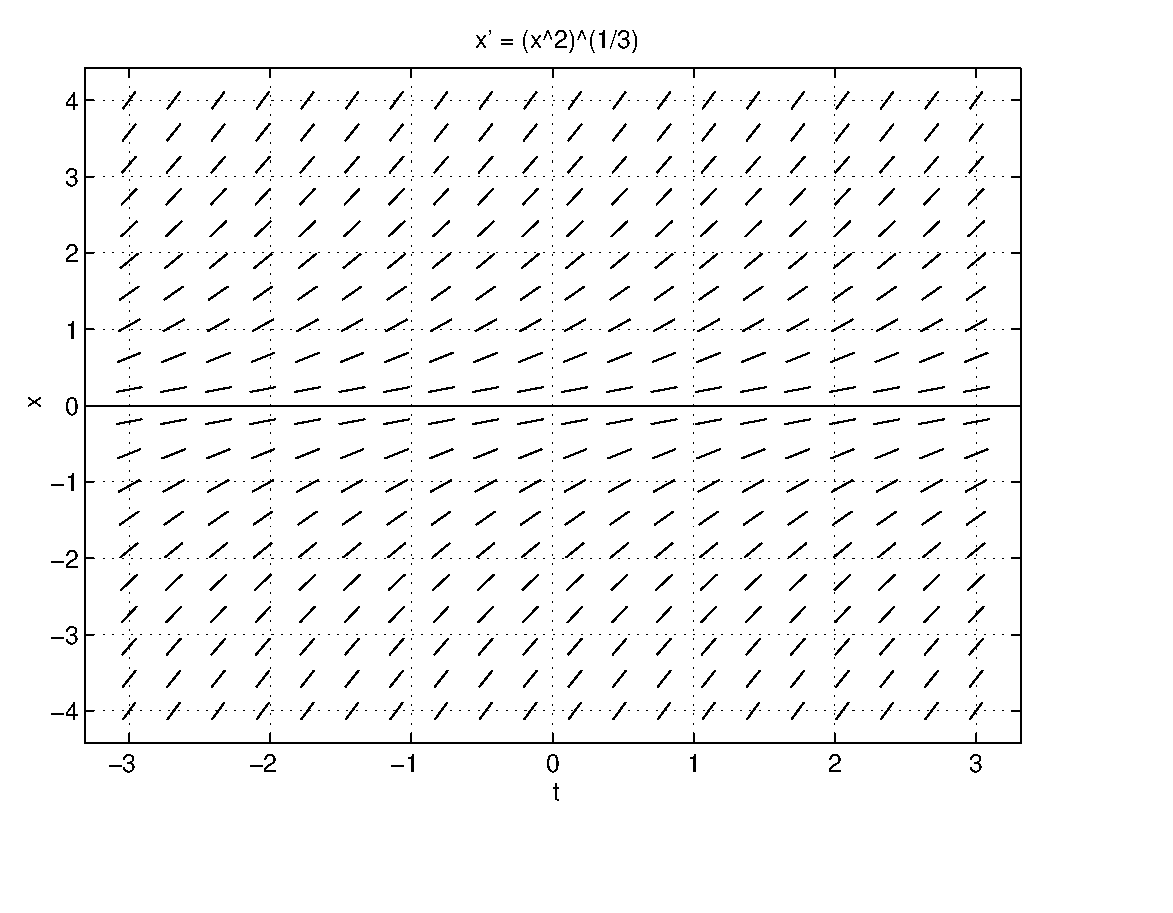
\psfig{file=figures/nonuniqa.eps,width=3.2in}
	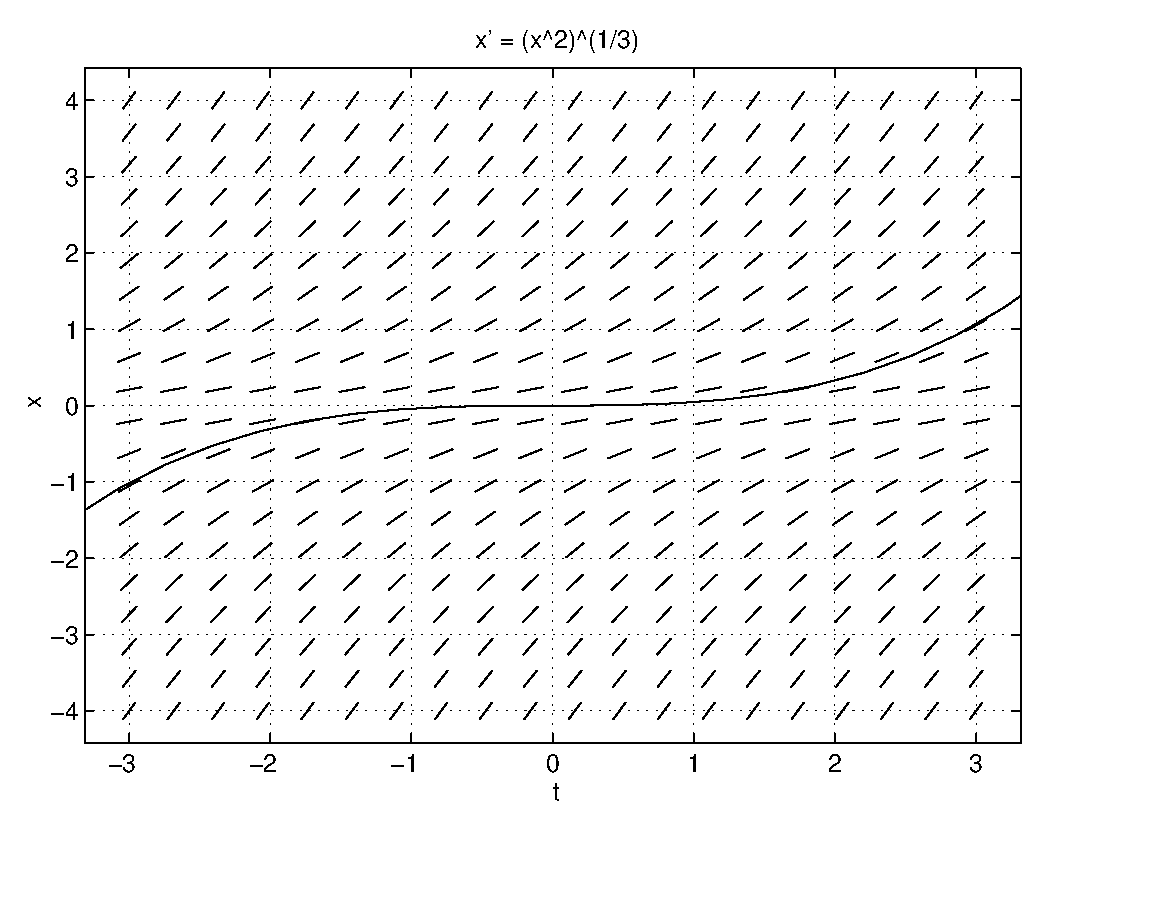
\psfig{file=figures/nonuniqb.eps,width=3.2in}}
        \caption{Solutions for \protect\Ref{nonunique}
              for $t\in [-3,3]$ and $x\in [-4,4]$. Left: $x(0)=0$.
	      Right: $x(0)=0.00001$.}
        \label{nonuniquefig}
\end{figure}

At this stage, we do not have the background to discuss the numerical
method employed by {\sf dfield5}.

\subsection*{The Initial Value Problem for Linear Systems}
\index{initial value problem}

In this chapter we discuss how to find solutions $(x(t),y(t))$ to
\Ref{2dlinsystem} satisfying the initial values $x(0)=x_0$ and $y(0)=y_0$.
It is convenient to rewrite \Ref{2dlinsystem} in matrix form as:
\begin{equation} \label{ndlinsystem}
\frac{dX}{dt}(t) = CX(t).
\end{equation}
The initial value problem is then stated as:  Find a solution to
\Ref{ndlinsystem} satisfying $X(0)=X_0$ where $X_0=(x_0,y_0)^t$.
Everything that we have said here works equally well for $n$
dimensional systems of linear differential equations.  Just let
$C$ be an $n\times n$ matrix and let $X_0$ be an $n$ vector
of initial conditions.

\subsubsection*{Solving the Initial Value Problem Using Superposition}

In Section~\ref{S:IVPR} we discussed how to solve~\Ref{ndlinsystem} when the
eigenvalues of $C$ are real and distinct.  Recall that when $\lambda_1$ and
$\lambda_2$ are distinct real eigenvalues of $C$ with associated
eigenvectors $v_1$ and $v_2$, there are two solutions to \Ref{ndlinsystem}
given by the explicit formulas
\[
X_1(t) = e^{\lambda_1 t}v_1 \AND X_2(t) = e^{\lambda_2 t}v_2.
\]
Superposition guarantees that every linear combination of these solutions
\[
X(t) = \alpha_1X_1(t)+\alpha_2X_2(t) =
\alpha_1e^{\lambda_1 t}v_1 + \alpha_2e^{\lambda_2 t}v_2
\]
is a solution to \Ref{ndlinsystem}.  In addition, we can always choose
scalars $\alpha_1,\alpha_2\in\R$ to solve any given initial value problem
of \Ref{ndlinsystem}.   It follows from the uniqueness of solutions to
initial value problems stated in Theorem~\ref{exist&unique} that all
solutions to \Ref{ndlinsystem} are included in this family of solutions.

We generalize this discussion so that we will be able to find closed form 
solutions to \Ref{ndlinsystem} in Section~\ref{S:TDM} when the eigenvalues 
of $C$ are complex or are real and equal.

Suppose that $X_1(t)$ and $X_2(t)$ are two solutions to \Ref{2dlinsystem} such
that
\[
v_1=X_1(0) \AND v_2=X_2(0)
\]
are linearly independent\index{linearly!independent}.  The existence part of
Theorem~\ref{exist&unique}
guarantees that such solutions exist.  Then all solutions to \Ref{2dlinsystem}
are linear combinations of these two solutions.  We verify this statement as
follows.  Corollary~\ref{C:dim=n} of Chapter~\ref{C:vectorspaces} states
that since $\{v_1,v_2\}$ is a linearly independent set in $\R^2$, it is
also a basis of $\R^2$.  Thus for every $X_0\in\R^2$ there exist scalars
$r_1,r_2$ such that
\[
X_0 = r_1v_1 + r_2v_2.
\]
It follows from superposition and Theorem~\ref{exist&unique} that the
solution
\[
X(t) = r_1X_1(t) + r_2X_2(t)
\]
is the unique solution whose initial condition vector is $X_0$.

We have proved that every solution to this linear system of differential
equations is a linear combination of these two solutions --- that is, we
have proved that the dimension of the space of solutions to \Ref{ndlinsystem}
is two.  This proof generalizes immediately to a proof of the following
theorem for $n\times n$ systems.

\begin{thm}  \label{T:solvends}
Let $C$ be an $n\times n$ matrix.  Suppose that $X_1(t),\ldots,X_n(t)$
are  solutions to $\dot{X}=CX$ such that the vectors of initial conditions
$v_j=X_j(0)$ are linearly independent in $\R^n$.  Then the unique solution
to the system \Ref{ndlinsystem} with initial condition $X(0)=X_0$ is
\begin{equation}  \label{E:genlsoln}
X(t)=r_1X_1(t) + \cdots + r_nX_n(t),
\end{equation}
where $r_1,\ldots,r_n$ are scalars satisfying
\begin{equation} \label{findscalars}
X_0 = r_1v_1 + \cdots + r_nv_n.
\end{equation}
\end{thm}\index{initial condition!linear independence}

We call \Ref{E:genlsoln} the {\em general solution\/} \index{general solution}
to the system of differential equations $\dot{X}=CX$.  When solving the
initial value problem we find a {\em particular solution\/}\index{particular
solution}
by specifying the scalars $r_1,\ldots,r_n$.

\begin{cor}  \label{C:indsoln}
Let $C$ be an $n\times n$ matrix and let ${\cal X}=\{X_1(t),\ldots,X_n(t)\}$
be solutions to the differential equation $\dot{X}=CX$ such that the vectors
$X_j(0)$ are linearly independent in $\R^n$.  Then the set of all solutions
to $\dot{X}=CX$ is an $n$-dimensional subspace of $(\CCone)^n$, and
${\cal X}$ is a basis for the solution subspace.
\end{cor}\index{subspace!of solutions}

Consider a special case of Theorem~\ref{T:solvends}.  Suppose that the
matrix $C$ has $n$ linearly independent eigenvectors $v_1,\ldots,v_n$ with
real eigenvalues $\lambda_1,\ldots,\lambda_n$.  Then the functions
$X_j(t)=e^{\lambda_j t}v_j$ are solutions to $\dot{X}=CX$.
Corollary~\ref{C:indsoln} implies that the functions $X_j$ form a basis for
the space of solutions of this system of differential equations.  Indeed,
the general solution to \Ref{ndlinsystem} is
\begin{equation}  \label{e:gensoln}
X(t) = r_1e^{\lambda_1 t}v_1 + \cdots + r_ne^{\lambda_n t}v_n.
\end{equation}
The particular solution that solves the initial value $X(0)=X_0$ is found by
solving \Ref{findscalars} for the scalars $r_1,\ldots,r_n$.





\EXER

\TEXER

\noindent In Exercises~\ref{c6.1.03a} -- \ref{c6.1.03d}, consider the system of
differential equations
\begin{equation} \label{Ex.1.03}
\begin{array}{rcr}
\frac{dx}{dt}  & = & 65x+42y \\
\frac{dy}{dt}  & = & -99x-64y.
\end{array}
\end{equation}
\begin{exercise} \label{c6.1.03a}
Verify that
\[
v_1 = \vectwo{2}{-3} \AND v_2 = \vectwo{-7}{11}
\]
are eigenvectors of the coefficient matrix of \Ref{Ex.1.03} and find
the associated eigenvalues.
\end{exercise}
\begin{exercise} \label{c6.1.03b}
Find the solution to \Ref{Ex.1.03} satisfying initial conditions $X(0) =
(-14,22)^t$.
\end{exercise}
\begin{exercise} \label{c6.1.03c}
Find the solution to \Ref{Ex.1.03} satisfying initial conditions $X(0) =
(-3,5)^t$.
\end{exercise}
\begin{exercise} \label{c6.1.03d}
Find the solution to \Ref{Ex.1.03} satisfying initial conditions $X(0) =
(9,-14)^t$.
\end{exercise}

\noindent In Exercises~\ref{c6.1.06a} -- \ref{c6.1.06d}, consider the system of
differential equations
\begin{equation} \label{Ex.1.06}
\begin{array}{rcr}
\frac{dx}{dt}  & = & x-y \\
\frac{dy}{dt}  & = & -x+y.
\end{array}
\end{equation}
\begin{exercise} \label{c6.1.06a}
The eigenvalues of the coefficient matrix of \Ref{Ex.1.06} are $0$ and $2$.
Find the associated eigenvectors.
\end{exercise}
\begin{exercise} \label{c6.1.06b}
Find the solution to \Ref{Ex.1.06} satisfying initial conditions
$X(0)=(2,-2)^t$.
\end{exercise}
\begin{exercise} \label{c6.1.06c}
Find the solution to \Ref{Ex.1.06} satisfying initial conditions
$X(0)=(2,6)^t$.
\end{exercise}
\begin{exercise} \label{c6.1.06d}
Find the solution to \Ref{Ex.1.06} satisfying initial conditions
$X(0)=(1,0)^t$.
\end{exercise}


\noindent In Exercises~\ref{c6.1.1a} -- \ref{c6.1.1d}, consider the system of
differential equations
\begin{equation} \label{E:c6.1.1}
\begin{array}{rcr}
\frac{dx}{dt}  & = & -y \\
\frac{dy}{dt}  & = &  x.
\end{array}
\end{equation}
\begin{exercise} \label{c6.1.1a}
Show that $(x_1(t),y_1(t)) = (\cos t,\sin t)$ is a solution to \Ref{E:c6.1.1}.
\end{exercise}
\begin{exercise} \label{c6.1.1b}
Show that $(x_2(t),y_2(t)) = (-\sin t,\cos t)$ is a solution to \Ref{E:c6.1.1}.
\end{exercise}
\begin{exercise} \label{c6.1.1c}
Using Exercises~\ref{c6.1.1a} and \ref{c6.1.1b}, find a solution $(x(t),y(t))$
to \Ref{E:c6.1.1} that satisfies $(x(0),y(0)) = (0,1)$.
\end{exercise}
\begin{exercise} \label{c6.1.1d}
Using Exercises~\ref{c6.1.1a} and \ref{c6.1.1b}, find a solution $(x(t),y(t))$
to \Ref{E:c6.1.1} that satisfies $(x(0),y(0)) = (1,1)$.
\end{exercise}

\noindent In Exercises~\ref{c6.1.2a} -- \ref{c6.1.2b}, consider the system of
differential equations
\begin{equation}  \label{E:c6.1.2}
\begin{array}{rcl}
\frac{dx}{dt} & = & -2x+7y \\
\frac{dy}{dt} & = &  5y,
\end{array}
\end{equation}
\begin{exercise} \label{c6.1.2a}
Find a solution to \Ref{E:c6.1.2}
satisfying the initial condition $(x(0),y(0)) = (1,0)$.
\end{exercise}
\begin{exercise} \label{c6.1.2b}
Find a solution to \Ref{E:c6.1.2}
satisfying the initial condition $(x(0),y(0)) = (-1,2)$.
\end{exercise}

\noindent In Exercises~\ref{c6.1.3a} -- \ref{c6.1.3c}, consider the matrix
\[
C = \left(\begin{array}{rrr} -1 & -10 & -6\\  0 & 4  & 3 \\  0  & -14  & -9
	\end{array}\right).
\]
\begin{exercise} \label{c6.1.3a}
Verify that
\[
v_1 = \left(\begin{array}{r} 1 \\ 0\\ 0\end{array}\right) \qquad
v_2 = \left(\begin{array}{r} 2 \\ -1\\ 2\end{array}\right) \quad \AND \quad
v_3 = \left(\begin{array}{r} 6 \\ -3\\ 7\end{array}\right)
\]
are eigenvectors of $C$ and find the associated eigenvalues.
\end{exercise}
\begin{exercise} \label{c6.1.3b}
Find a solution to the system of differential equations
$\dot{X}=CX$ satisfying the initial condition $X(0)= (10, -4, 9)^t$.
\end{exercise}
\begin{exercise} \label{c6.1.3c}
Find a solution to the system of differential equations
$\dot{X}=CX$ satisfying the initial condition $X(0)= ( 2, -1, 3)^t$.
\end{exercise}

\begin{exercise}  \label{c6.1.4A}
Show that for some nonzero $a$ the function $x(t)=at^5$ is a solution to the
differential equation $\dot{x}=x^{4/5}$.  Then show that there are at least
two solutions to the initial value problem $x(0)=0$ for this differential
equation.
\end{exercise}


\CEXER

\begin{exercise} \label{c6.1.4}
Use {\sf pplane5}\index{\computer!pplane5} to investigate the system
of differential equations
\begin{equation}  \label{Ex.1.4}
\begin{array}{rcr}
\frac{dx}{dt}  & = & -2y \\
\frac{dy}{dt}  & = &  -x+y.
\end{array}
\end{equation}
\begin{itemize}
\item[(a)] Use {\sf pplane5} to find two independent eigendirections (and
hence eigenvectors) for \Ref{Ex.1.4}.
\item[(b)] Using (a), find the eigenvalues of the coefficient matrix of
\Ref{Ex.1.4}.
\item[(c)] Find a closed form solution to \Ref{Ex.1.4} satisfying the initial
condition
\[
X(0) = \vectwo{4}{-1}.
\]
\item[(d)] Study the time series of $y$ versus $t$ for the solution in (c)
by comparing the graph of the closed form solution obtained in (c) with the
time series graph using {\sf pplane5}.
\end{itemize}
\end{exercise}




\Section{Closed Form Solutions by the Direct Method}
\label{S:TDM}


In Section~\ref{S:IVPR} we showed in detail how solutions to planar systems
of constant coefficient differential equations with distinct real eigenvalues
are found.  This method was just reviewed in Section~\ref{S:6.1} where we saw
that the crucial step in solving these systems of differential equations is
the step where we find two linearly independent solutions.   In this section
we discuss how to find these two linearly independent solutions when the
eigenvalues of the coefficient matrix are either complex or real and equal.

By finding these two linearly independent solutions we will find both
the {\em general\/} solution of the system of differential equations
$\dot{X}=CX$ and a method for solving the initial value
problem\index{initial value problem}
\begin{equation}  \label{e:eqnA}
\begin{array}{rcl}
\dps\frac{dX}{dt} & = & CX\\
X(0) & = & X_0.
\end{array}
\end{equation}
We assume that $C$ is a $2\times 2$ matrix with eigenvalues $\lambda_1$ and
$\lambda_2$.  When needed, we denote the associated eigenvectors by $v_1$ and
$v_2$.

\subsection*{Real Distinct Eigenvalues}
\index{eigenvalue!real}

We have discussed the case when $\lambda_1\neq\lambda_2\in\R$ on several
occasions.  For completeness we repeat the result.  The general solution is:
\begin{equation}  \label{E:RD2}
X(t) = \alpha_1 e^{\lambda_1 t}v_1 + \alpha_2 e^{\lambda_2 t}v_2.
\end{equation}
The initial value problem is solved by finding real numbers $\alpha_1$ and
$\alpha_2$ such that
\[
X_0 = \alpha_1 v_1 + \alpha_2 v_2.
\]
See Section~\ref{S:IVPR} for a detailed discussion with examples.

\subsection*{Complex Conjugate Eigenvalues}
\index{eigenvalue!complex}

Suppose that the eigenvalues of $C$ are complex, that is, suppose that
$\lambda_1= \sigma+i\tau$ with $\tau\neq 0$ is an eigenvalue of $C$ with
eigenvector $v_1=v+iw$, where $v,w\in\R^2$.  We claim that
$X_1(t)$ and $X_2(t)$, where
\begin{equation}  \label{E:CC1}
\begin{array}{rcl}
X_1(t) & = & e^{\sigma t}(\cos(\tau t)v -\sin(\tau t)w)\\
X_2(t) & = & e^{\sigma t}(\sin(\tau t)v +\cos(\tau t)w),
\end{array}
\end{equation}
are solutions to \Ref{e:eqnA} and that the general
solution\index{general solution} to \Ref{e:eqnA} is:
\begin{equation}  \label{E:CC2}
X(t) = \alpha_1 X_1(t) + \alpha_2 X_2(t),
\end{equation}
where $\alpha_1, \alpha_2$ are real scalars.

There are several difficulties in deriving \Ref{E:CC1} and \Ref{E:CC2}; these
difficulties are related to using complex numbers as opposed to real numbers.
In particular, in the derivation of \Ref{E:CC1} we need to define the
exponential of a complex number, and we begin by discussing this issue.

\subsubsection*{Euler's Formula}\index{Euler's formula}

We find complex exponentials by using Euler's celebrated formula:
\begin{equation}  \label{E:Euler}
e^{i\theta} = \cos\theta + i\sin\theta
\end{equation}
for any real number $\theta$.  A justification of this formula is
given in Exercise~\ref{c6.6.05}.   Euler's formula allows us to differentiate
complex exponentials, obtaining the expected result:
\begin{eqnarray*}
\frac{d}{dt}e^{i\tau t} & = &
\frac{d}{dt}(\cos(\tau t) + i\sin(\tau t))\\
& = & \tau(-\sin(\tau t) + i\cos(\tau t)) \\
& = & i\tau(\cos(\tau t) + i\sin(\tau t))\\
& = & i\tau e^{i\tau t}.
\end{eqnarray*}

Euler's formula also implies that
\begin{equation}  \label{E:ecis}
e^{\lambda t} = e^{\sigma t + i\tau t} = e^{\sigma t}e^{i\tau t} =
e^{\sigma t}(\cos(\tau t) + i\sin(\tau t)),
\end{equation}
where $\lambda = \sigma+i\tau$.  Most importantly, we note that
\begin{equation}  \label{E:eldiff}
\frac{d}{dt}e^{\lambda t} = \lambda e^{\lambda t}.
\end{equation}
We use \Ref{E:ecis} and the product rule for differentiation to verify
\Ref{E:eldiff} as follows:
\begin{eqnarray*}
\frac{d}{dt}e^{\lambda t} & =  &
\frac{d}{dt}\left(e^{\sigma t}e^{i\tau t}\right)\\
& = & \left(\sigma e^{\sigma t}\right)e^{i\tau t}
+ e^{\sigma t}\left(i\tau e^{i\tau t}\right)\\
& = & (\sigma+i\tau)e^{\sigma t + i\tau t} \\
& = & \lambda e^{\lambda t}.
\end{eqnarray*}

\subsubsection*{Verification that \protect\Ref{E:CC2} is the General Solution}

A complex vector-valued function $X(t)=X_1(t)+iX_2(t)\in\C^n$
\index{complex valued solution} consists of
a {\em real part\/} $X_1(t)\in\R^n$ and an {\em imaginary part\/}
\index{complex valued solution!real part}
\index{complex valued solution!imaginary part}
$X_2(t)\in\R^n$.  For such functions $X(t)$ we define
\[
\dot{X} = \dot{X}_1+i\dot{X}_2
\]
and
\[
CX = CX_1 + iCX_2.
\]
To say that $X(t)$ is a solution to $\dot{X}=CX$ means that
\begin{equation}  \label{E:X1X2}
\dot{X}_1+i\dot{X}_2 = \dot{X} = CX = CX_1 + iCX_2.
\end{equation}

\begin{lemma}  \label{L:RIsoln}
The complex vector-valued function $X(t)$ is a solution to $\dot{X}=CX$ if
and only if the real and imaginary parts are real vector-valued solutions
to $\dot{X}=CX$.
\end{lemma}

\proof Equating the real and imaginary parts of \Ref{E:X1X2} implies that
\[
\dot{X}_1 = CX_1 \AND \dot{X}_2 = CX_2.
\]
\qed

It follows from Lemma~\ref{L:RIsoln} that finding one complex-valued solution
to a linear differential equation provides us with two real-valued solutions.
Identity \Ref{E:eldiff} implies that
\[
X(t) = e^{\lambda_1 t}v_1
\]
is a complex-valued solution to \Ref{e:eqnA}.  Using Euler's formula we
compute the real and imaginary parts of $X(t)$, as follows.
\begin{eqnarray*}
X(t) & = & e^{(\sigma+i\tau)t}(v+iw) \\
& = & e^{\sigma t} (\cos(\tau t)+i\sin(\tau t))(v+iw)\\
& = & e^{\sigma t}(\cos(\tau t)v-\sin(\tau t)w)+
ie^{\sigma t}(\sin(\tau t)v+\cos(\tau t)w).
\end{eqnarray*}
Since the real and imaginary parts of $X(t)$ are solutions to $\dot{X}=CX$, it
follows that the real-valued functions $X_1(t)$ and $X_2(t)$ defined in
\Ref{E:CC1} are indeed solutions.

Returning to the case where $C$ is a $2\times 2$ matrix, we see that if
$X_1(0)=v$ and $X_2(0)=w$ are linearly independent, then
Corollary~\ref{C:indsoln} implies that \Ref{E:CC2} is the general solution to
$\dot{X}=CX$.  The linear independence of $v$ and $w$ is verified using the
following lemma.

\begin{lemma}  \label{L:rievind}
Let $\lambda_1=\sigma+i\tau$ with $\tau\neq 0$ be a
complex eigenvalue\index{eigenvalue!complex} of the
$2\times 2$ matrix $C$ with eigenvector\index{eigenvector}
$v_1=v+iw$ where $v,w\in\R^2$.  Then
\begin{equation}  \label{e:complexcoord}
\begin{array}{rcl}
Cv & = & \sigma v - \tau w \\
Cw & = & \tau v + \sigma w.
\end{array}
\end{equation}
and $v$ and $w$ are linearly independent\index{linearly!independent} vectors.
\end{lemma}

\proof   By assumption $Cv_1=\lambda_1v_1$, that is,
\begin{equation}  \label{E:viw}
C (v+iw) = (\sigma+i\tau)(v+iw) = (\sigma v - \tau w) + i(\tau v + \sigma w).
\end{equation}
Equating real and imaginary parts of \Ref{E:viw} leads to the system of
equations \Ref{e:complexcoord}.  Note that if $w=0$, then $v\neq 0$ and
$\tau v = 0$.  Hence $\tau=0$, contradicting the assumption that
$\tau\neq 0$.  So $w\neq 0$.

Note also that if $v$ and $w$ are linearly dependent, then $v=\alpha w$.
It then follows from the previous equation that
\[
Cw = (\tau\alpha+\sigma)w.
\]
Hence $w$ is a real eigenvector; but the eigenvalues of $C$ are not real and
$C$ has no real eigenvectors.   \qed


\subsubsection*{An Example with Complex Eigenvalues}

Consider an example of an initial value problem for a linear system with
complex eigenvalues.  Let
\begin{equation}  \label{e:complexexample}
\frac{dX}{dt} = \mattwo{-1}{2}{-5}{-3} X = CX,
\end{equation}
and
\[
X_0=\vectwo{1}{1}.
\]

The characteristic polynomial\index{characteristic polynomial} for the
matrix $C$ is:
\[
p_C(\lambda) = \lambda^2 +4\lambda + 13,
\]
whose roots are $\lambda_1 = -2+3i$ and $\lambda_2 = -2-3i$. So
\[
\sigma = -2 \AND \tau = 3.
\]
An eigenvector corresponding to the eigenvalue $\lambda_1$ is
\[
v_1 = \vectwoc{2}{-1+3i} = \vectwo{2}{-1}+i\vectwo{0}{3}=v+iw.
\]
It follows from \Ref{E:CC1} that
\[
\begin{array}{rcl}
X_1(t) & = & e^{-2t}(\cos(3t)v -\sin(3t)w)\\
X_2(t) & = & e^{-2t}(\sin(3t)v +\cos(3t)w),
\end{array}
\]
are solutions to \Ref{e:complexexample} and $X=\alpha_1X_1+\alpha_2X_2$ is
the general solution to \Ref{e:complexexample}.  To solve the initial value
problem we need to find $\alpha_1,\alpha_2$ such that
\[
X_0 = X(0) = \alpha_1X_1(0) + \alpha_2X_2(0) = \alpha_1 v + \alpha_2 w,
\]
that is,
\[
\vectwo{1}{1} = \alpha_1\vectwo{2}{-1}  + \alpha_2\vectwo{0}{3}.
\]
Therefore, $\alpha_1 = \frac{1}{2}$ and $\alpha_2=\frac{1}{2}$ and
\begin{equation}  \label{e:complexexampleans}
X(t) =  e^{-2t}\vectwoc{\cos(3t)+\sin(3t)}{\cos(3t)-2\sin(3t)}.
\end{equation}

\subsection*{Real and Equal Eigenvalues}

There are two types of $2\times 2$ matrices that have real and equal
\index{eigenvalue!real!equal}
eigenvalues --- those that are scalar multiples of the identity and those
that are not.  An example of a $2\times 2$ matrix that has real and equal
eigenvalues is
\begin{equation}  \label{E:equalex}
A = \mattwoc{\lambda_1}{1}{0}{\lambda_1}, \quad \lambda_1\in\R.
\end{equation}
The characteristic polynomial of $A$ is
\[
p_A(\lambda) = \lambda^2 - \trace(A)\lambda + \det(A) =
\lambda^2 -2\lambda_1\lambda + \lambda_1^2 = (\lambda-\lambda_1)^2.
\]
Thus the eigenvalues of $A$ both equal $\lambda_1$.

\subsubsection*{Only One Linearly Independent Eigenvector}

An important fact about the matrix $A$ in \Ref{E:equalex} is that it has
only one linearly independent eigenvector.  To verify this fact, solve the
system of linear equations
\[
Av = \lambda_1v.
\]
In matrix form this equation is
\[
0 = (A-\lambda_1I_2)v = \mattwo{0}{1}{0}{0}v.
\]
A quick calculation shows that all solutions are multiples of
$v_1=e_1=(1,0)^t$.

In fact, this observation is valid for any $2\times 2$ matrix that has
equal eigenvalues and is not a scalar multiple of the identity, as the next
lemma shows.

\begin{lemma}  \label{L:1indeig}
Let $A$ be a $2\times 2$ matrix.  Suppose that $A$ has two linearly
independent eigenvectors both with eigenvalue $\lambda_1$.
Then $A=\lambda_1 I_2$.
\end{lemma}\index{eigenvector!linearly independent}\index{eigenvector!real}

\proof  Let $v_1$ and $v_2$ be two linearly independent
eigenvectors of $A$, that is, $Av_j = \lambda_1 v_j$.  It follows
from linearity that $Av=\lambda_1 v$ for any linear combination
$v=\alpha_1v_1+\alpha_2v_2$.  Since $v_1$ and $v_2$ are linearly
independent and $\dim(\R^2)=2$, it follows that $\{v_1,v_2\}$ is
a basis of $\R^2$.  Thus, every vector $v\in\R^2$ is a linear
combination of $v_1$ and $v_2$.  Therefore, $A$ is $\lambda_1$ times
the identity matrix.  \qed

\subsubsection*{Generalized Eigenvectors}

Suppose that $C$ has exactly one linearly independent real eigenvector $v_1$
with real eigenvalue $\lambda_1$.  We call $w_1$ a {\em generalized
eigenvector\/}\index{eigenvector!generalized} of $C$ it satisfies the
system of linear equations
\begin{equation} \label{e:Cw=lw+va}
(C-\lambda_1I_2)w_1 = v_1.
\end{equation}

The matrix $A$ in \Ref{E:equalex} has a generalized eigenvector. To verify
this point solve the linear system
\[
(A-\lambda_1I_2)w_1 = \mattwo{0}{1}{0}{0}w_1 = v_1 = \vectwo{1}{0}
\]
for $w_1=e_2$.   Note that for this matrix $A$, $v_1=e_1$ and $w_1=e_2$ are
linearly independent.  The next lemma shows that this observation about
generalized eigenvectors is always valid.

\begin{lemma}  \label{L:geneig2}
Let $C$ be a $2\times 2$ matrix with both eigenvalues equal to $\lambda_1$
and with one linearly independent eigenvector $v_1$.  

\noindent (a)  Let $w_1$ be a generalized eigenvector of $C$, then $v_1$ and 
$w_1$ are linearly independent. 

\noindent (b)  Let $w$ be any vector such that $v_1$ and $w$ are linearly 
independent.  Then $w$ is a nonzero scalar multiple of a generalized 
eigenvector of $C$.
\end{lemma}

\proof  (a) If $v_1$ and $w_1$ were linearly dependent, then $w_1$ would be 
a multiple of $v_1$ and hence an eigenvector of $C$.  But $C-\lambda_1I_2$
applied to an eigenvector is zero, which is a contradiction.  Therefore, 
$v_1$ and $w_1$ are linearly independent.

(b) Let $w$ be any vector that is linearly independent of
the eigenvector $v_1$.  It follows that  $\{v_1,w\}$ is a basis for
$\R^2$; hence
\begin{equation} \label{E:Cw1}
Cw = \alpha v_1 + \beta w
\end{equation}
for some scalars $\alpha$ and $\beta$.    If $\alpha=0$, then
$w$ is an eigenvector of $C$, contradicting the assumption that $C$ has
only one linearly independent eigenvector.  Therefore, $\alpha\neq 0$.

We claim that $\beta=\lambda_1$ and we prove the claim by showing that
$\beta$ is an eigenvalue of $C$.  Hence $\beta$ must equal $\lambda_1$
since both eigenvalues of $C$ equal $\lambda_1$.  To see that $\beta$
is an eigenvalue, define the nonzero vector
\[
u = \alpha v_1 +(\beta-\lambda_1)w
\]
and compute
\[
Cu = \lambda_1 \alpha v_1 + (\beta-\lambda_1)(\alpha v_1+\beta w) =
\beta u.
\]
So $u$ is an eigenvector of $C$ with eigenvalue $\beta$.
It now follows from \Ref{E:Cw1} that
\[
(C-\lambda_1I_2)w = \alpha v_1.
\]
Therefore, $w_1=\frac{1}{\alpha}w$ is a generalized eigenvector
of $C$.  \qed



\subsubsection*{Independent Solutions to Differential Equations with
Equal Eigenvalues}

In the equal eigenvalue one eigenvector case, we
claim that the general solution\index{general solution} to $\dot{X}=CX$ is:
\begin{equation}  \label{e:exp1eva}
X(t) = e^{\lambda_1 t}\left(\alpha v_1 +\beta (w_1+tv_1)\right),
\end{equation}
where $v_1$ is an eigenvector of $C$ and $w_1$ is the generalized
eigenvector.

Since $v_1$ is an eigenvector of $C$ with eigenvalue $\lambda_1$, the
function $X_1(t)=e^{\lambda_1 t}v_1$ is a solution to $\dot{X}=CX$.  Suppose
that we can show that $X_2(t)=e^{\lambda_1 t}(w_1+tv_1)$ is also a solution
to $\dot{X}=CX$.  Then \Ref{e:exp1eva} is the general solution, since
$X_1(0)=v_1$ and $X_2(0)=w_1$ are linearly independent by 
Lemma~\ref{L:geneig2}(a).  Apply Theorem~\ref{T:solvends}.

To verify that $X_2(t)$ is a solution (that is, that $\dot{X}_2=CX_2$),
calculate
\[
\dot{X}_2(t) = \lambda_1 e^{\lambda_1 t}(w_1+tv_1) + e^{\lambda_1 t}v_1=
e^{\lambda_1 t}(\lambda_1 w_1 + v_1 +t\lambda v_1)
\]
and
\[
CX_2(t) = e^{\lambda_1 t}(Cw_1+tCv_1) = e^{\lambda_1 t}
((v_1+\lambda_1 w_1)+t\lambda_1 v_1),
\]
using \Ref{e:Cw=lw+va}.  Note that $X(0)=\alpha v_1 + \beta w_1$, so $\alpha$
and $\beta$ are found by solving $X_0= \alpha v_1 + \beta w_1$.

\subsubsection*{An Example with Equal Eigenvalues}

Consider the system of differential equations
\begin{equation}  \label{e:shearexample}
\frac{dX}{dt} = \mattwo{1}{-1}{9}{-5} X
\end{equation}
with initial value
\[
X_0 = \vectwo{2}{3}.
\]
The characteristic polynomial for the matrix $C=\mattwo{1}{-1}{9}{-5}$ is
\[
p_C(\lambda) = \lambda^2 + 4\lambda +4 = (\lambda + 2)^2.
\]
Thus $\lambda_1=-2$ is an eigenvalue of multiplicity two.  Since
$C$ is not a multiple of the identity matrix, it must have
precisely one linearly independent eigenvector $v_1$.  This eigenvector is
found by solving the equation
\[
0 = (C-\lambda_1I_2)v_1 = (C+2I_2)v_1 = \mattwo{3}{-1}{9}{-3}v_1
\]
for
\[
v_1=\vectwo{1}{3}.
\]
To find the generalized eigenvector $w_1$, we solve the system of linear
equations
\[
(C-\lambda_1I_2)w_1=(C+2I_2)w_1=\mattwo{3}{-1}{9}{-3}w_1= v_1=\vectwo{1}{3}
\]
by row reducing the augmented matrix
\[
\left(\begin{array}{rr|r} 3 & -1 & 1\\ 9 & -3 & 3 \end{array}\right)
\]
to obtain
\[
w_1 = \vectwo{1}{2}.
\]

We may now apply \Ref{e:exp1eva} to find the general solution to
\Ref{e:shearexample}
\[
X(t) = e^{-2t}\left(\alpha v_1 +\beta (w_1+tv_1)\right).
\]
We solve the initial value problem by solving
\[
\vectwo{2}{3} = X_0 = X(0) = \alpha v_1 +\beta w_1 =
\mattwo{1}{1}{3}{2}\vectwo{\alpha}{\beta}
\]
for $\alpha=-1$ and $\beta=3$.   So the closed form solution to this initial
value problem is
\begin{eqnarray*}
X(t) & = & e^{-2t}\left(-v_1 + 3(w_1+tv_1)\right)\\
& = & e^{-2t}\left(-\vectwo{1}{3}+3\vectwoc{1+t}{2+3t}\right)\\
& = & e^{-2t}\vectwo{2+3t}{3+9t}.
\end{eqnarray*}

There is a simpler method for finding this solution --- a method that
does not require solving for either the eigenvector $v_1$ or the generalized
eigenvector $w_1$ that we will discuss later.  See Section~\ref{S:6.6}.

\EXER

\TEXER

\begin{exercise}  \label{c6.6.05}
Justify Euler's formula \Ref{E:Euler} as follows.  Recall the
Taylor series
\begin{eqnarray*}
e^x & = & 1 + x + \frac{1}{2!}x^2 + \cdots + \frac{1}{n!}x^n + \cdots\\
\cos x & = & 1 - \frac{1}{2!}x^2 + \frac{1}{4!}x^4 + \cdots +
(-1)^n \frac{1}{(2n)!}x^{2n} + \cdots \\
\sin x & = & x - \frac{1}{3!}x^3 + \frac{1}{5!}x^5 + \cdots +
(-1)^n \frac{1}{(2n+1)!}x^{2n+1} + \cdots.
\end{eqnarray*}
Now evaluate the Taylor series $e^{i\theta}$ and separate into real and
imaginary parts.
\end{exercise}

 In modern language De Moivre's formula states that
\[
e^{ni\theta} = \left(e^{i\theta}\right)^n.
\]
In Exercises~\ref{c6.6.1a} -- \ref{c6.6.1b} use De Moivre's formula coupled
with Euler's formula \Ref{E:Euler} to determine trigonometric identities
for the given quantity in terms of $\cos\theta$, $\sin\theta$, $\cos\varphi$,
$\sin\varphi$.
\begin{exercise}  \label{c6.6.1a}
$\cos(\theta+\varphi)$.
\end{exercise}
\begin{exercise}  \label{c6.6.1b}
$\sin(3\theta)$.
\end{exercise}

In Exercises~\ref{c6.6.2a} -- \ref{c6.6.2d} compute the general solution for
the given system of differential equations.
\begin{exercise}  \label{c6.6.2a}
$\dps\frac{dX}{dt} = \mattwo{-1}{-4}{2}{3} X$.
\end{exercise}
\begin{exercise}  \label{c6.6.2b}
$\dps\frac{dX}{dt} = \mattwo{8}{-15}{3}{-4} X$.
\end{exercise}
\begin{exercise}  \label{c6.6.2c}
$\dps\frac{dX}{dt} = \mattwo{5}{-1}{1}{3} X$.
\end{exercise}
\begin{exercise}  \label{c6.6.2d}
$\dps\frac{dX}{dt} = \mattwo{-4}{4}{-1}{0} X$.
\end{exercise}

\Section{Solutions Using Matrix Exponentials}
\label{S:Matrixexp} \index{matrix!exponential}

In Section~\ref{S:growthmodels} we showed that the solution of the single
ordinary differential equation $\dot x(t) = \lambda x(t)$ with initial
condition $x(0)=x_0$ is $x(t) = e^{t\lambda}x_0$ (see \Ref{lin1} in
Chapter~\ref{chap:SolveOdes}).  In this section we show that we
may write solutions of systems of equations in a similar form.
In particular, we show that the solution to the linear system of ODEs
\begin{equation}   \label{eq:x=Mx}
\frac{dX}{dt} = CX
\end{equation}
with initial condition
\[
X(0) = X_0,
\]
where $C$ is an $n\times n$ matrix and $X_0\in\R^n$, is
\begin{equation}  \label{matrixsoln}
X(t) = e^{tC}X_0.
\end{equation}

In order to make sense of the solution \Ref{matrixsoln} we need
to understand matrix exponentials. More precisely, since $tC$ is
an $n\times n$ matrix for each $t\in\R$, we need to make sense
of the expression $e^L$ where $L$ is an $n\times n$ matrix.  For
this we recall the form of the exponential function as a power
series:
\[
     e^t = 1 + t + \frac{1}{2!} t^2 + \frac{1}{3!} t^3
     + \frac{1}{4!} t^4 + \cdots .
\]
In more compact notation we have
\[
     e^t = \sum\limits_{k=0}^\infty \frac{1}{k!} t^k.
\]
By analogy, define the {\em matrix exponential\/}\index{matrix!exponential}
$e^L$ by
\begin{eqnarray}
e^{L} & = & I_n + L + \frac{1}{2!} L^2 + \frac{1}{3!} L^3 +\cdots
\label{e:expL}\\
      & = & \sum\limits_{k=0}^\infty\frac{1}{k!} L^k. \nonumber
\end{eqnarray}
In this formula $L^2 = LL$ is the matrix product of $L$ with itself, and the
power $L^k$ is defined inductively by $L^k = LL^{k-1}$ for $k>1$.  Hence
$e^L$ is an $n\times n$ matrix and is the infinite sum of $n\times n$
matrices.

\noindent {\bf Remark:}   The infinite series for matrix exponentials
\Ref{e:expL} does converge for all $n\times n$ matrices $L$, and this fact
is proved in Exercises~\ref{c6.2.7} and \ref{c6.2.8}.

Using \Ref{e:expL}, we can write the matrix exponential of $tC$
for each real number $t$.  Since $(tC)^k = t^k C^k$ we obtain
\arraystart
\begin{equation}  \label{eq:MatrixExp}
\begin{array}{rcl}
\dps e^{tC} & = & \dps I_n + tC + \frac{1}{2!} (tC)^2 + \frac{1}{3!} (tC)^3
+\cdots\\
\dps & = & \dps I_n + tC + \frac{t^2}{2!} C^2 + \frac{t^3}{3!} C^3 +\cdots.
\end{array}
\end{equation}
\arrayfinish
Next we claim that
\begin{equation}  \label {e:diffmatexp}
  \frac{d}{dt} e^{tC} = Ce^{tC}.
\end{equation}
We verify the claim by supposing that we can differentiate
\Ref{eq:MatrixExp} term by term with respect to $t$. Then
\begin{eqnarray*}
  \dps\frac{d}{dt} e^{tC} & = & \frac{d}{dt}(I_n) + \frac{d}{dt}(tC)
  + \frac{d}{dt}\left(\frac{t^2}{2!} C^2\right) +
  \frac{d}{dt}\left(\frac{t^3}{3!} C^3\right) +
  \frac{d}{dt}\left(\frac{t^4}{4!}C^4\right) + \cdots\\
     & = & 0 + C + t C^2 + \frac{t^2}{2!} C^3 +
\frac{t^3}{3!} C^4 + \cdots\\
     & = & C\left(I_n + tC + \frac{t^2}{2!} C^2 + \frac{t^3}{3!} C^3
+\cdots\right)\\
     & = & Ce^{tC}.
\end{eqnarray*}
It follows that the function $X(t) = e^{tC}X_0$ is a solution of
\Ref{eq:x=Mx} for each $X_0\in\R^n$; that is,
\[
     \frac{d}{dt} X(t) =  \frac{d}{dt}  e^{tC}X_0
     = C e^{tC}X_0 = C X(t).
\]
Since \Ref{e:expL} implies that $e^{0C} = e^0 = I_n$, it follows
that $X(t) = e^{tC}X_0$ is a solution of \Ref{eq:x=Mx} with
initial condition $X(0)=X_0$.  This discussion shows that solving
\Ref{eq:x=Mx} in closed form is equivalent to finding a closed
form expression for the matrix exponential $e^{tC}$.

\begin{thm}  \label{T:linODEsoln}
The unique solution\index{uniqueness of solutions} to the
initial value problem\index{initial value problem}
\arraystart
\[
\begin{array}{rcl}
\dps\frac{dX}{dt} & = & CX \\
X(0) & = & X_0
\end{array}
\]
\arrayfinish
is
\[
X(t)=e^{tC}X_0.
\]
\end{thm}

\proof  Existence follows from the previous discussion;
uniqueness follows from the $n$ dimensional analog of
Theorem~\ref{exist&unique}.  \qed


\subsection*{Explicit Computation of Matrix Exponentials}
\index{matrix!exponential!computation}

We begin with the simplest computation of a matrix exponential.

\noindent (a) \quad Let $L$ be a multiple of the identity; that
is, let $L = \alpha I_n$ where $\alpha$ is a real number.  Then
\begin{equation} \label{ex:expm}
e^{\alpha I_n} = e^{\alpha} I_n.
\end{equation}
That is, $e^{\alpha I_n}$ is a scalar multiple of the
identity.  To verify \Ref{ex:expm}, compute
\[
e^{\alpha I_n} = I_n + \alpha I_n + \frac{\alpha^2}{2!} I_n^2 +
\frac{\alpha^3}{3!} I_n^3 +\cdots = (1+\alpha+\frac{\alpha^2}{2!}
+\frac{\alpha^3}{3!}+\cdots)I_n = e^{\alpha} I_n.
\]

\noindent (b) \quad Let $C$ be a $2\times 2$ diagonal matrix,
     \[
          C = \mattwo{\lambda_1}{0}{0}{\lambda_2},
     \]
where $\lambda_1$ and $\lambda_2$ are real constants.  Then
\begin{equation}  \label{e:expdiag}
e^{tC} = \mattwo{e^{\lambda_1 t}}{0}{0}{e^{\lambda_2 t}}.
\end{equation}
To verify \Ref{e:expdiag} compute
\begin{eqnarray*}
   e^{tC} & = & I_2 + tC + \frac{t^2}{2!} C^2 +  \frac{t^3}{3!} C^3 +\cdots\\
        & = & \mattwo{1}{0}{0}{1} + \mattwo{\lambda_1 t}{0}{0}{\lambda_2 t} +
\mattwo{\frac{t^2}{2!}\lambda_1^2}{0}{0}{\frac{t^2}{2!}\lambda_2^2} +\cdots\\
        & = & \mattwo{e^{\lambda_1 t}}{0}{0}{e^{\lambda_2 t}}.
\end{eqnarray*}

\noindent (c) \quad Suppose that
     \[
                C = \mattwo{0}{-1}{1}{0}.
      \]
Then
\begin{equation} \label{e:exprotate}
e^{tC} = \mattwo{\cos t}{-\sin t}{\sin t}{\cos t}.
\end{equation}
We begin this computation by observing that
\[
C^2 = -I_2, \quad C^3 = -C, \AND C^4 = I_n.
\]
Therefore, by collecting terms of odd and even power in the series
expansion for the matrix exponential we obtain
\begin{eqnarray*}
e^{tC} & = & I_2 + tC + \frac{t^2}{2!} C^2 +  \frac{t^3}{3!}C^3 +\cdots\\
     & = & I_2 + tC - \frac{t^2}{2!}I_2 - \frac{t^3}{3!}C +\cdots\\
     & = & \left(1 - \frac{t^2}{2!} + \frac{t^4}{4!} - \frac{t^6}{6!} +
		\cdots \right)I_2
	 + \left(t - \frac{t^3}{3!} + \frac{t^5}{5!} - \frac{t^7}{7!} +
	\cdots \right)C \\
     & = & (\cos t)I_2 + (\sin t)C \\
     & = & \mattwo{\cos t}{-\sin t}{\sin t}{\cos t}.
     \end{eqnarray*}
In this computation we have used the fact that the trigonometric
functions $\cos t$ and $\sin t$ have the power series expansions:
\begin{eqnarray*}
\cos t & = & 1-\frac{1}{2!}t^2+\frac{1}{4!} t^4 + \cdots =
\sum\limits_{k=0}^\infty\frac{(-1)^k}{(2k)!} t^{2k},\\
\sin t & = & t-\frac{1}{3!} t^3 + \frac{1}{5!} t^5 + \cdots
   = \sum\limits_{k=0}^\infty \frac{(-1)^k}{(2k+1)!} t^{2k+1}.
\end{eqnarray*}
See Exercise~\ref{c6.2.5C} for an alternative proof of \Ref{e:exprotate}.

To compute the matrix exponential
\Matlab\index{matrix!exponential!in \protect\Matlab} provides the command
{\tt expm}\index{\computer!expm}.  We use this command to compute
the matrix exponential $e^{tC}$ for
\[
C=\mattwo{0}{-1}{1}{0} \AND t=\frac{\pi}{4}.
\]
Type
\begin{verbatim}
C = [0, -1; 1, 0];
t = pi/4;
expm(t*C)
\end{verbatim}
that gives the answer
\begin{verbatim}
ans =
    0.7071   -0.7071
    0.7071    0.7071
\end{verbatim}
Indeed, this is precisely what we expect by \Ref{e:exprotate},
since
\[
\cos\left(\frac{\pi}{4}\right)=\sin\left(\frac{\pi}{4}\right)=
\frac{1}{\sqrt{2}}\approx 0.70710678.
\]

\noindent (d) \quad Let
\[
C = \mattwo{0}{1}{0}{0}.
\]
Then
\begin{equation}  \label{e:nilpotent}
e^{tC} = I_2 + tC = \mattwo{1}{t}{0}{1},
\end{equation}
since $C^2=0$.

\EXER

\CEXER

\begin{exercise} \label{c6.2.1}
Let $L$ be the $3\times 3$ matrix
\[
     L = \left(\begin{array}{rrr}
    2 & 0 & -1\\
    0 & -1 & 3\\
    1 & 0 & 1
               \end{array}\right).
\]
Find the smallest integer $m$ such that
\[
  I_3+L+\frac{1}{2!} L^2 + \frac{1}{3!} L^3 + \cdots
  + \frac{1}{m!} L^m
\]
is equal to $e^L$ up to a precision of two decimal places.  More
exactly, use the \Matlab command {\tt expm} to compute $e^L$ and
use \Matlab commands to compute the series expansion to order $m$.  Note
that the command for computing $n!$ in \Matlab is
{\tt prod(1:n)}\index{\computer!prod}.
\end{exercise}

\begin{exercise} \label{c6.2.2}
Use \Matlab to compute the matrix exponential $e^{tC}$ for
\[
     C =\mattwo{1}{1}{2}{-1}
\]
by choosing for $t$ the values $1.0,1.5$ and $2.5$.  Does $e^{C}
e^{1.5C}=e^{2.5C}$?
\end{exercise}

\begin{exercise} \label{c6.2.3}
For the scalar exponential function $e^{t}$ it is well known
that for any pair of real numbers $t_1,t_2$ the following
equality holds:
\[
     e^{t_1+t_2} = e^{t_1}e^{t_2}.
\]
Use \Matlab to find two $2\times 2$ matrices $C_1$ and $C_2$ such that
\[
     e^{C_1+C_2} \not= e^{C_1}e^{C_2}.
\]
\end{exercise}

\TEXER

\noindent In Exercises~\ref{c6.2.4a} -- \ref{c6.2.4c} compute the matrix
exponential $e^{tC}$ for the matrix.
\begin{exercise} \label{c6.2.4a}
                $\mattwo{0}{1}{0}{0}$.
\end{exercise}
\begin{exercise} \label{c6.2.4b}
                $\left(\begin{array}{ccc}
                0 & 1 & 0\\
                0 & 0 & 1\\
                0 & 0 & 0 \end{array}\right)$.
\end{exercise}
\begin{exercise} \label{c6.2.4c}
                $\mattwo{0}{-2}{2}{0}$.
\end{exercise}

\begin{exercise} \label{c6.2.5}
Let $\alpha,\beta$ be real numbers and let $\alpha I$ and $\beta
I$ be corresponding $n\times n$ diagonal matrices.  Use
properties of the scalar exponential function to show that
\[
     e^{(\alpha + \beta)I} = e^{\alpha I}e^{\beta I}.
\]
\end{exercise}

\noindent In Exercises~\ref{c6.2.5A} -- \ref{c6.2.5C} we use
Theorem~\ref{exist&unique}, the uniqueness of solutions to initial value
problems, in perhaps a surprising way.
\begin{exercise}  \label{c6.2.5A}
Prove that
\[
e^{t+s} = e^te^s
\]
for all real numbers $s$ and $t$.  {\bf Hint:}
\begin{itemize}
\item[(a)]  Fix $s$ and verify that $y(t) = e^{t+s}$ is a solution to the
initial value problem
\begin{equation}  \label{E:init1}
\begin{array}{rcl}
\frac{dx}{dt} & = & x \\
x(0) & = & e^s
\end{array}
\end{equation}
\item[(b)] Fix $s$ and verify that $z(t) = e^te^s$ is also a solution to
\Ref{E:init1}.
\item[(c)]  Use Theorem~\ref{exist&unique} to conclude that $y(t)=z(t)$ for
every $s$.
\end{itemize}
\end{exercise}
\begin{exercise}  \label{c6.2.5B}
Let $A$ be an $n\times n$ matrix.  Prove that
\[
e^{(t+s)A} = e^{tA}e^{sA}
\]
for all real numbers $s$ and $t$.  {\bf Hint:}
\begin{itemize}
\item[(a)]  Fix $s\in\R$ and $X_0\in\R^n$ and verify that
$Y(t) = e^{(t+s)A}X_0$ is a solution to the initial value problem
\begin{equation}  \label{E:init2}
\begin{array}{rcl}
\frac{dX}{dt} & = & AX \\
X(0) & = & e^{sA}X_0
\end{array}
\end{equation}
\item[(b)] Fix $s$ and verify that $Z(t) = e^{tA}\left(e^{sA}X_0\right)$ is
also a solution to \Ref{E:init2}.
\item[(c)]  Use the $n$ dimensional version of Theorem~\ref{exist&unique} to
conclude that $Y(t)=Z(t)$ for every $s$ and every $X_0$.
\end{itemize}
{\bf Remark:}  Compare the result in this exercise with the calculation in
Exercise~\ref{c6.2.5}.
\end{exercise}
\begin{exercise}  \label{c6.2.5C}
Prove that
\begin{equation}  \label{E:0-110E}
\exp\left(t\mattwo{0}{-1}{1}{0}\right) =
\mattwo{\cos t}{-\sin t}{\sin t}{\cos t}.
\end{equation}
{\bf Hint:}
\begin{itemize}
\item[(a)] Verify that $X_1(t) = \vectwo{\cos t}{\sin t}$ and
$X_2(t) = \vectwo{-\sin t}{\cos t}$ are solutions to the initial value problems
\begin{equation}  \label{E:init3}
\begin{array}{rcl}
\dps\frac{dX}{dt} & = & \mattwo{0}{-1}{1}{0}X \\
X(0) & = & e_j
\end{array}
\end{equation}
for $j=1,2$.
\item[(b)] Since $X_j(0)=e_j$, use Theorems~\ref{exist&unique} and
\ref{T:linODEsoln} to verify that
\begin{equation}   \label{E:0-110}
X_j(t) = \exp\left(t\mattwo{0}{-1}{1}{0}\right)e_j.
\end{equation}
\item[(c)]  Show that \Ref{E:0-110} proves \Ref{E:0-110E}
\end{itemize}
\end{exercise}

\begin{exercise}  \label{c6.2.6A}
Let $C$ be an $n\times n$ matrix.  Use Theorem~\ref{T:linODEsoln} to show
that the $n$ columns of the $n\times n$ matrix $e^{tC}$ give a basis of
solutions for the system of differential equations $\dot{X}=CX$.
\end{exercise}

\noindent {\bf Remark:}  The completion of Exercises~\ref{c6.2.7} and
\ref{c6.2.8} constitutes a proof that the infinite series definition of
the matrix exponential is a convergent series for all $n\times n$ matrices.

\begin{exercise}  \label{c6.2.7}
Let $A=(a_{ij})$ be an $n\times n$ matrix.  Define
\[
||A||_m = \max_{1\leq i\leq n} (|a_{i1}|+\cdots+|a_{in}|)
= \max_{1\leq i\leq n} \left(\sum_{j=1}^n|a_{ij}|\right).
\]
That is, to compute $||A||_m$, first sum the absolute values of the entries
in each row of $A$, and then take the maximum of these sums.  Prove that:
\[
||AB||_m \leq ||A||_m ||B||_m.
\]
{\bf Hint:} Begin by noting that
\[
||AB||_m =
\max_{1\leq i\leq n}\left(\sum_{j=1}^n\left|\sum_{k=1}^na_{ik}b_{kj}\right|
\right)\leq \max_{1\leq i\leq n}\left(\sum_{j=1}^n\sum_{k=1}^n\left|a_{ik}b_{kj}
\right|\right) = \max_{1\leq i\leq n}\left(\sum_{k=1}^n\sum_{j=1}^n
\left|a_{ik}b_{kj}\right|\right).
\]
\end{exercise}

\begin{exercise} \label{c6.2.8}
Recall that an infinite series of real numbers
\[
c_1+c_2 +\cdots+c_N + \cdots
\]
converges absolutely if there is a constant $K$ such that for every $N$
the partial sum satisfies:
\[
|c_1| + |c_2| + \cdots + |c_N| \leq K.
\]

Let $A$ be an $n\times n$ matrix.  To prove that the matrix exponential $e^A$
is an absolutely convergent infinite series use Exercise~\ref{c6.2.7} and the
following steps.  Let $a_N$ be the $(i,j)^{th}$ entry in the matrix $A^N$
where $A^0=I_n$.
\begin{itemize}
\item[(a)]  $|a_N| \leq ||A^N||_m$.
\item[(b)]  $||A^N||_m \leq ||A||_m^N$.
\item[(c)]  $|a_0| + |a_1| + \cdots + \frac{1}{N!}|a_N| \leq e^{||A||_m}$.
\end{itemize}
\end{exercise}


\Section{Linear Normal Form Planar Systems} \index{normal form}
\label{S:LNFPS}

There are three linear systems of ordinary differential equations
that we now solve explicitly using matrix exponentials.  Remarkably,
in a sense to be made precise, these are the only linear planar systems.
The three systems are listed in Table~\ref{T:3sys}.


\begin{table}[htb]
\begin{center}
\begin{tabular}{|c|c|c|}
\hline
name  & equations & closed form solution \\
\hline
(a) & $\dot{X} = \mattwo{\lambda_1}{0}{0}{\lambda_2} X$ &
$X(t) = \mattwo{e^{\lambda_1 t}}{0}{0}{e^{\lambda_2 t}}X_0$ \\
\hline
(b) & $\dot{X}=\mattwo{\sigma}{-\tau}{\tau}{\sigma}X$ & $X(t) = e^{\sigma t}
\mattwo{\cos(\tau t)}{-\sin(\tau t)}{\sin(\tau t)}{\cos(\tau t)}X_0$\\
\hline
(c) & $\dot{X} = \mattwo{\lambda_1}{1}{0}{\lambda_1}$ &
$X(t) = e^{\lambda_1 t}\mattwo{1}{t}{0}{1}X_0$ \\
\hline
\end{tabular}
\caption{Solutions to normal form ODEs with $X(0)=X_0$.}
\label{T:3sys}
\end{center}
\end{table}

The verification of Table~\ref{T:3sys}(a) follows from \Ref{e:expdiag}, but
it just reproduces earlier work in Section~\ref{sec:UncoupledLS} where we
considered uncoupled systems of two ordinary differential equations.
To verify the solutions to (b) and (c), we need to prove:

\begin{prop}  \label{P:expAB}
Let $A$ and $B$ be two $n\times n$ matrices such that
\begin{equation} \label{e:AB=BA}
AB = BA.
\end{equation}
Then
\[
e^{A+B} = e^A e^B.
\]
\end{prop} \index{matrix!exponential}

\proof  Note that \Ref{e:AB=BA} implies that
\begin{eqnarray}
A^kB    & = & BA^k  \label{e:AkB=BAk}\\
e^{tA}B & = & Be^{tA}. \label{e:etAB=BetA}
\end{eqnarray}
Identity \Ref{e:AkB=BAk} is verified when $k=2$ using
associativity of matrix multiplication, as follows
\[
A^2B = AAB = ABA = BAA = BA^2.
\]
The argument for general $k$ is identical.  Identity
\Ref{e:etAB=BetA} follows directly from \Ref{e:AkB=BAk} and
the power series definition of matrix exponentials \Ref{e:expL}.

We use Theorem~\ref{exist&unique}  to complete the proof of this
proposition.  Recall that
\[
X(t) = e^{t(A+B)}X_0
\]
is the unique solution to the initial value problem
\begin{eqnarray*}
\frac{dX}{dt} & = & (A+B)X \\ \\
X(0) & = & X_0.
\end{eqnarray*}
We claim that
\[
Y(t) = e^{tA}e^{tB}X_0
\]
is another solution to this equation.  Certainly $Y(0)=X_0$.  It
follows from \Ref{e:diffmatexp} that
\[
\frac{d}{dt}e^{tA} = Ae^{tA} \AND \frac{d}{dt}e^{tB} = Be^{tB}.
\]
Thus the product rule together with \Ref{e:etAB=BetA} imply that
\begin{eqnarray*}
\frac{dY}{dt} & = & \left(Ae^{tA}\right)e^{tB}X_0 +
e^{tA}\left(Be^{tB}\right)X_0 \\
& = & (A+B) e^{tA} e^{tB} X_0\\
& = & (A+B)Y(t).
\end{eqnarray*}
Thus
\[
\frac{dY}{dt} = (A+B)Y,
\]
and $Y(t)=X(t)$.  Since $X_0$ is arbitrary it follows that
\[
e^{t(A+B)} = e^{tA}e^{tB}.
\]
Evaluating at $t=1$ yields the desired result.  \qed

\subsubsection{Verification of Table~\protect{\ref{T:3sys}}(b)}

We begin by noting that the $2\times 2$ matrix $C$ in (b) is
\[
C = \mattwo{\sigma}{-\tau}{\tau}{\sigma} = \sigma I_2 + \tau J,
\]
where
\[
J= \mattwo{0}{-1}{1}{0}.
\]
Since $I_2J=JI_2$, it follows from Proposition~\ref{P:expAB} that
\[
e^{tC} = e^{(\sigma t)I_2} e^{(\tau t)J}.
\]
Thus \Ref{ex:expm} and \Ref{e:exprotate} imply
\begin{equation}  \label{e:exprotation}
e^{tC} = e^{\sigma t}
\mattwo{\cos(\tau t)}{-\sin(\tau t)}{\sin(\tau t)}{\cos(\tau t)},
\end{equation}
and (b) is verified.

\subsubsection{Verification of Table~\protect{\ref{T:3sys}}(c)}

To determine the solutions to Table~\ref{T:3sys}(c), observe that
\[
C = \mattwoc{\lambda_1}{1}{0}{\lambda_1} = \lambda_1 I_2 + N,
\]
where
\[
N = \mattwo{0}{1}{0}{0}.
\]
Since $I_2N=NI_2$, Proposition~\ref{P:expAB} implies
\begin{equation}  \label{e:expshear}
e^{tC} = e^{(t\lambda_1)I_2}e^{tN} =
e^{t\lambda}\mattwo{1}{t}{0}{1}
\end{equation}
by \Ref{ex:expm} and \Ref{e:nilpotent}.

\subsubsection{Summary}

The normal form matrices in Table~\ref{T:3sys} are characterized by the number
of linearly independent real eigenvectors.  We summarize this information in
Table~\ref{T:3sysa}.  We show, in Section~\ref{S:6.5}, that any planar
linear system of ODEs can be solved just by noting how many independent
eigenvectors the corresponding matrix has; general solutions are found by
transforming the equations into one of the three types of equations
listed in Table~\ref{T:3sys}.

\begin{table}[htb]
\begin{center}
\begin{tabular}{|c|c|c|}
\hline
Matrix  & Number of Real Eigenvectors & Reference \\
\hline
 $\mattwoc{\lambda_1}{0}{0}{\lambda_2}$ & two linearly independent  &
Section~\ref{S:IVPR} \\
\hline
$\mattwo{\sigma}{-\tau}{\tau}{\sigma}$ & none
& Chapter~\ref{chap:SolveOdes}, \Ref{E:cmplxnf} \\
\hline
$\mattwoc{\lambda_1}{1}{0}{\lambda_1}$ &  one linearly independent
& Lemma~\ref{L:1indeig} \\
\hline
\end{tabular}
\caption{Number of linearly independent real eigenvectors.}
\label{T:3sysa}
\end{center}
\end{table}


\EXER

\TEXER

\begin{exercise} \label{c6.3.1}
Solve the initial value problem
\[
\begin{array}{rcr}
\dot{x} & = & 2x + 3y \\
\dot{y} & = & -3x + 2y
\end{array}
\]
where $x(0) = 1  \AND  y(0) = -2$.
\end{exercise}

\begin{exercise} \label{c6.3.2}
Solve the initial value problem
\[
\begin{array}{rcr}
\dot{x} & = & -2x + y \\
\dot{y} & = & -2y
\end{array}
\]
where $x(0) = 4  \AND y(0) = -1$.
\end{exercise}

\begin{exercise} \label{c6.3.25}
Let $A$ be an $n\times n$ matrix such that $A^3=0$.  Compute $e^{tC}$
where $C=2I_n+A$.
\end{exercise}

\CEXER

\begin{exercise} \label{c6.3.3}
Use {\sf pplane5} to plot phase plane portraits for each of the
three types of linear systems (a), (b) and (c) in Table~\ref{T:3sys}.
Based on this computer exploration answer the following questions:
\begin{itemize}
\item[(i)]  If a solution to that system spirals about the origin,
is the system of differential equations of type (a), (b) or (c)?
\item[(ii)]  How many eigendirections are there for equations of type (c)?
\item[(iii)]  Let $(x(t),y(t))$ be a solution to one of these three types of
systems and suppose that $y(t)$ oscillates up and down infinitely often.
Then $(x(t),y(t))$ is a solution for which type of system?
\end{itemize}
\end{exercise}



\Section{Similar Matrices} \label{S:6.5}

In Section~\ref{S:LNFPS} we discussed solutions to differential equations
$\dot{X}=CX$ for three classes of matrices $C$.  See Table~\ref{T:3sys}.
We stated that in a certain sense every $2\times 2$ matrix can be
thought of as a member of one of these families.  In this section we
show that every $2\times 2$ matrix is similar to one of the matrices in that
table (see Theorem~\ref{T:putinform}), where similarity is defined as follows.

\begin{Def}  \label{D:similar}
The $n\times n$ matrices $B$ and $C$ are {\em similar\/} if
there exists an invertible $n\times n$ matrix $P$ such that
\[
C = P\inv BP.
\]
\end{Def} \index{similar}\index{similar!matrices} \index{invertible}

Our present interest in similar matrices stems from the fact that if we
know the solutions to the system of differential equations $\dot{Y}=CY$ in
closed form, then we know the solutions to the system of differential
equations $\dot{X}=BX$ in closed form.  More precisely,
\begin{lemma}  \label{L:simsoln}
Suppose that $B$ and $C=P\inv BP$ are similar matrices.  If
$Y(t)$ is a solution to the system of differential equations
$\dot{Y}=CY$, then $X(t)=PY(t)$ is a solution to the system of 
differential equations $\dot{X}=BX$.
\end{lemma}

\proof   Since the entries in the matrix $P$ are constants, it follows that
\[
\frac{dX}{dt} = P\frac{dY}{dt}.
\]
Since $Y(t)$ is a solution to the $\dot{Y}=CY$ equation, it follows that
\[
\frac{dX}{dt} = PCY.
\]
Since $Y=P\inv X$ and $PCP\inv = B$,
\[
\frac{dX}{dt} = PCP\inv X = BX.
\]
Thus $X(t)$ is a solution to $\dot{X}=BX$, as claimed.  \qed


\subsection*{Invariants of Similarity}

\begin{lemma}  \label{L:simdettr}
Let $A$ and $B$ be similar $2\times 2$ matrices.  Then
\begin{eqnarray*}
p_A(\lambda) & = & p_B(\lambda),\\
\det(A) & = & \det(B),\\
\trace(A) & = & \trace(B),
\end{eqnarray*} \index{characteristic polynomial}\index{trace}
and the eigenvalues of $A$ and $B$ are equal.
\end{lemma}

\proof
The determinant\index{determinant} is a function on $2\times 2$ matrices
that has several important properties.  Recall, in particular, from
Chapter~\ref{chap:matrices}, Theorem~\ref{propdet} that for any pair of
$2\times 2$ matrices $A$ and $B$:
\begin{equation} \label{e:detprod}
\det(AB) =  \det(A)\det(B),
\end{equation}
and for any invertible $2\times 2$ matrix $P$
\begin{equation}  \label{e:detinv}
\det(P\inv)  =  \frac{1}{\det(P)}.
\end{equation}

Let $P$ be an invertible $2\times 2$ matrix so that $B=P\inv AP$.
Using \Ref{e:detprod} and \Ref{e:detinv} we see that
\begin{eqnarray*}
p_B(\lambda) & = & \det(B-\lambda I_2) \\
 & = & \det(P\inv AP-\lambda I_2) \\
& = & \det(P\inv(A-\lambda I_2)P) \\
& = & \det(A-\lambda I_2) \\
& = & p_A(\lambda).
\end{eqnarray*}
Hence the eigenvalues of $A$ and $B$ are the same.  It follows
from \Ref{e:treigen} and \Ref{e:deteigen} of Section~\ref{S:evchp}
that the determinants and traces of $A$ and $B$ are equal.   \qed

For example, if
\[
A = \mattwo{-1}{0}{0}{1} \AND  P = \mattwo{1}{2}{1}{1},
\]
then
\[
P\inv = \mattwo{-1}{2}{1}{-1}
\]
and
\[
P\inv AP = \mattwo{3}{4}{-2}{-3}.
\]
A calculation shows that
\[
\det(P\inv AP)=-1=\det(A) \AND {\rm tr}(P\inv AP)=0={\rm tr}(A),
\]
as stated in Lemma~\ref{L:simdettr}.


\subsubsection*{Similarity and Matrix Exponentials}

We introduce similarity at this juncture for the following reason:
if $C$ is a matrix that is similar to $B$, then $e^C$ can be computed
from $e^B$.  More precisely:

\begin{lemma} \label{L:similarexp}
Let $C$ and $B$ be $n\times n$ similar matrices, and let $P$ be
an invertible $n\times n$ matrix such that
\[
C=P\inv BP.
\]
Then
\begin{equation}  \label{e:similarexp}
e^C = P\inv e^BP.
\end{equation}
\end{lemma} \index{similar} \index{invertible}

\proof Note that for all powers of $k$ we have
\[
(P\inv BP)^k = P\inv B^kP.
\]
Next verify \Ref{e:similarexp} by computing
\[
e^C =\sum^{\infty}_{k=0} \frac{1}{k!}C^k
 =  \sum^{\infty}_{k=0} \frac{1}{k!}(P\inv BP)^k
=  \sum^{\infty}_{k=0} \frac{1}{k!}P\inv B^kP
= P\inv\left(\sum^{\infty}_{k=0} \frac{1}{k!}B^k\right)P
= P\inv e^B P.
\]
\qed


\subsection*{Classification of $2\times 2$ Matrices}
\index{normal form}

We now classify all $2\times 2$ matrices up to similarity.

\begin{thm}  \label{T:putinform}
Let $C$ and $P=(v_1|v_2)$ be $2\times 2$ matrices where the vectors
$v_1$ and $v_2$ are specified below.
\begin{itemize}
\item[(a)]	Suppose that $C$ has two linearly independent
real eigenvectors $v_1$ and $v_2$ with real eigenvalues $\lambda_1$
and $\lambda_2$.  Then
\[
P\inv CP = \mattwoc{\lambda_1}{0}{0}{\lambda_2}.
\]

\item[(b)]	Suppose that $C$ has no real eigenvectors and
complex conjugate eigenvalues $\sigma\pm i\tau$ where
$\tau\neq 0$.  Then
\[
P\inv CP = \mattwo{\sigma}{-\tau}{\tau}{\sigma},
\]
where $v_1 + iv_2$ is an eigenvector of $C$ associated with the
eigenvalue $\lambda_1=\sigma-i\tau$.

\item[(c)]	Suppose that $C$ has exactly one linearly
independent real eigenvector $v_1$ with real eigenvalue $\lambda_1$.
Then
\[
P\inv CP = \mattwoc{\lambda_1}{1}{0}{\lambda_1},
\]
where  $v_2$ is a generalized eigenvector of $C$ that satisfies
\begin{equation}  \label{e:Cw=lw+v}
(C-\lambda_1 I_2) v_2 =  v_1.
\end{equation}

\end{itemize}
\end{thm}

\proof
The strategy in the proof of this theorem is to determine the
$1^{st}$ and $2^{nd}$ columns of $P\inv CP$ by computing (in each case)
$P\inv CPe_j$ for $j=1$ and $j=2$.  Note from the definition of $P$
that
\[
Pe_1 = v_1 \AND Pe_2 = v_2.
\]
In addition, if $P$ is invertible, then
\[
P\inv v_1 = e_1 \AND P\inv v_2 = e_2.
\]
Note that if $v_1$ and $v_2$ are linearly independent, then $P$ is invertible.

(a) \quad Since $v_1$ and $v_2$ are assumed to be linearly independent,
$P$ is invertible.  So we can compute
\[
P\inv CPe_1 = P\inv C v_1 = \lambda P\inv v_1 = \lambda e_1.
\]
It follows that the $1^{st}$ column of $P\inv CP$	is
\[
\vectwoc{\lambda_1}{0}.
\]
Similarly, the $2^{nd}$ column of $P\inv CP$ is
\[
\vectwoc{0}{\lambda_2}
\]
thus verifying (a).

(b) \quad  Lemma~\ref{L:rievind} implies that $v_1$ and $v_2$ are linearly
independent and hence that $P$ is invertible.  Using \Ref{e:complexcoord},
with $\tau$ replaced by $-\tau$, $v$ replaced by $v_1$, and $w$ replaced by
$w_1$, we calculate
\[
P\inv CPe_1 = P\inv Cv_1 = \sigma P\inv v_1 + \tau P\inv v_2
= \sigma e_1 + \tau e_2,
\]
and
\[
P\inv CPe_2 = P\inv Cv_2 = -\tau P\inv v_1 + \sigma P\inv v_2
= -\tau e_1 + \sigma e_2.
\]
Thus the columns of $P\inv CP$ are
\[
\vectwo{\sigma}{\tau} \AND \vectwo{-\tau}{\sigma},
\]
as desired.


(c) \quad   Let $v_1$ be an eigenvector and assume that $v_2$ is a
generalized eigenvector satisfying \Ref{e:Cw=lw+v}.  By
Lemma~\ref{L:geneig2} the vectors $v_1$ and $v_2$ exist and are linearly
independent.

For this choice of $v_1$ and $v_2$, compute
\[
P\inv CPe_1 = P\inv Cv_1 = \lambda_1 P\inv v_1 = \lambda_1 e_1,
\]
and
\[
P\inv CPe_2 = P\inv Cv_2 = P\inv v_1+\lambda_1 P\inv v_2 = e_1+\lambda_1 e_2.
\]
Thus the two columns of $P\inv CP$ are:
\[
\vectwoc{\lambda_1}{0} \AND \vectwoc{1}{\lambda_1}.
\]
  \qed


\subsection*{Closed Form Solutions Using Similarity}
\index{closed form solution}

We now use Lemma~\ref{L:simsoln}, Theorem~\ref{T:putinform}, and the
explicit solutions to the normal form equations Table~\ref{T:3sys}
to find solutions for $\dot{X}=CX$ where $C$ is any $2\times 2$ matrix.
The idea behind the use of similarity to solve systems of ODEs is to
transform a given system into another normal form system whose solution is
already known.  This method is very much like the technique of change of
variables used when finding indefinite integrals in calculus.

We suppose that we are given a system of differential equations $\dot{X}=CX$
and use Theorem~\ref{T:putinform} to transform $C$ by similarity to one of
the normal form matrices listed in that theorem.  We then solve the
transformed equation, as we did in Section~\ref{S:LNFPS} (see
Table~\ref{T:3sys}), and use Lemma~\ref{L:simsoln} to transform the solution
back to the given system.

For example, suppose that $C$ has a complex eigenvalue $\sigma-i\tau$ with
corresponding eigenvector $v+iw$.  Then Theorem~\ref{T:putinform} states that
\[
B = P\inv CP = \mattwo{\sigma}{-\tau}{\tau}{\sigma},
\]
where $P=(v|w)$ is an invertible matrix.  Using Table~\ref{T:3sys} the
general solution to the system of equations $\dot{Y}=BY$ is:
\[
Y(t) = e^{\sigma t}
\mattwo{\cos(\tau t)}{-\sin(\tau t)}{\sin(\tau t)}{\cos(\tau t)}
\vectwo{\alpha}{\beta}.
\]
Lemma~\ref{L:simsoln} states that
\[
X(t) = PY(t)
\]
is the general solution to the $\dot{X}=CX$ system.  Moreover, we can solve
the initial value problem by solving
\[
X_0 = PY(0) = P\vectwo{\alpha}{\beta}
\]
for $\alpha$ and $\beta$.  In particular,
\[
\vectwo{\alpha}{\beta} = P\inv X_0.
\]
Putting these steps together implies that
\begin{equation} \label{e:exp0ev}
X(t) = e^{\sigma t}
P\mattwo{\cos(\tau t)}{-\sin(\tau t)}{\sin(\tau t)}{\cos(\tau t)}P\inv X_0
\end{equation}
is the solution to the initial value problem.

\subsubsection*{The Example with Complex Eigenvalues Revisited}
\index{eigenvalue!complex}

Recall the example in \Ref{e:complexexample}
\[
\frac{dX}{dt} = \mattwo{-1}{2}{-5}{-3} X,
\]
with initial values
\[
X_0=\vectwo{1}{1}.
\]
This linear system has a complex eigenvalue $\sigma-i\tau=-2-3i$ with
corresponding eigenvector
\[
v+iw = \vectwoc{2}{-1-3i}.
\]
Thus the matrix $P$ that transforms $C$ into normal form is
\[
P = \mattwo{2}{0}{-1}{-3} \AND P\inv = \frac{1}{6}\mattwo{3}{0}{-1}{-2}.
\]
It follows from \Ref{e:exp0ev} that the solution to the initial value problem
is
\begin{eqnarray*}
X(t) & =  &
e^{-2t}P\mattwo{\cos(3t)}{-\sin(3t)}{\sin(3t)}{\cos(3t)}P\inv X_0 \\ & = &
\frac{1}{6}e^{-2t}\mattwo{2}{0}{-1}{-3}
\mattwo{\cos(3t)}{-\sin(3t)}{\sin(3t)}{\cos(3t)}
\mattwo{3}{0}{-1}{-2}\vectwo{1}{1}.
\end{eqnarray*}
A calculation gives
\begin{eqnarray*}
X(t) & = & \frac{1}{2}e^{-2t}\mattwo{2}{0}{-1}{-3}
\mattwo{\cos(3t)}{-\sin(3t)}{\sin(3t)}{\cos(3t)}\vectwo{1}{-1}  \\
& = & e^{-2t}
\vectwoc{\cos(3t)+\sin(3t)}{\cos(3t)-2\sin(3t)}.
\end{eqnarray*}
Thus the solution to \Ref{e:complexexample} that we have found using 
similarity of matrices is identical to the solution \Ref{e:complexexampleans}
that we found by the direct method.

Solving systems with either distinct real eigenvalues or equal eigenvalues
works in a similar fashion.



\EXER

\TEXER

\begin{exercise} \label{c6.5.1}
Suppose that the matrices $A$ and $B$ are similar and the matrices
$B$ and $C$ are similar.  Show that $A$ and $C$ are also similar
matrices.
\end{exercise}

\begin{exercise} \label{c6.5.2}
Use \Ref{e:trAB=trBA} in Chapter~\ref{chap:matrices} to verify that the
traces of similar matrices are equal.
\end{exercise}

\noindent In Exercises~\ref{c6.5.3a} -- \ref{c6.5.3b} determine whether
or not the given matrices are similar, and why.
\begin{exercise} \label{c6.5.3a}
$A = \mattwo{1}{2}{3}{4} \AND B = \mattwo{2}{-2}{-3}{8}$.
\end{exercise}
\begin{exercise} \label{c6.5.3b}
$C = \mattwo{2}{2}{2}{2} \AND D = \mattwo{4}{-2}{-2}{4}$.
\end{exercise}

\begin{exercise} \label{c6.5.4}
Let $B=P\inv AP$ so that $A$ and $B$ are similar matrices.  Suppose
that $v$ is an eigenvector of $B$ with eigenvalue $\lambda$.  Show
that $Pv$ is an eigenvector of $A$ with eigenvalue $\lambda$.
\end{exercise}

\begin{exercise} \label{c6.5.5}
Which $n\times n$ matrices are similar to $I_n$?
\end{exercise}

\begin{exercise} \label{c6.5.6}
Compute $e^A$ where
\[
A = \mattwo{3}{-1}{1}{1}.
\]
Check your answer using \Matlabp.
\end{exercise}


\Sec{*Formulas for Matrix Exponentials}{FORMULAS FOR MATRIX EXPONENTIALS}
%\Section{Formulas for Matrix Exponentials} 
\label{S:6.6}
\index{closed form solution}\index{matrix!exponential!computation}

We now complete our discussion of exact solutions to planar linear systems of
ODEs $\dot{X}=CX$.  There are three different methods for finding closed form
solutions to systems of ODEs.  We have discussed two of these methods.  In
the first we find solutions by the direct method, that is, we find two linear
independent solutions whose linear combinations form the space of solutions.
See Section~\ref{S:TDM}.  In the second method we use similarity and normal
form equations (whose solutions are obtained using matrix exponentials) to
find closed form solutions.  See Sections~\ref{S:LNFPS} and \ref{S:6.5}.
In this section we present a third method based on computable formulas for
matrix exponentials derived using the Cayley Hamilton theorem.

\subsection*{A Formula for the Matrix Exponential}

For $2\times 2$ matrices $C$ with eigenvalues $\lambda_1$ and $\lambda_2$
there is a simple formula for the matrix exponential $e^{tC}$ whose
derivation depends on the Cayley Hamilton theorem. \index{Cayley Hamilton
theorem}  When the eigenvalues $\lambda_1$ and $\lambda_2$ of $C$ are
distinct, the formula is
\begin{equation}  \label{E:exdist}
e^{tC} = \frac{1}{\lambda_2-\lambda_1}\left(e^{\lambda_1 t}(C-\lambda_2I_2) -
e^{\lambda_2 t}(C-\lambda_1I_2)\right).
\end{equation}
When the eigenvalues are equal, the formula is
\begin{equation}  \label{E:exeq}
e^{tC} = e^{\lambda_1 t}(I_2 + tN)
\end{equation}
where $N = C - \lambda_1I_2$.

Note that when computing the matrix exponential using either \Ref{E:exdist}
or \Ref{E:exeq}, it is not necessary to compute the eigenvectors of $C$.
This is a substantial simplification.  But it is with the use of formula
\Ref{E:exeq} that the greatest simplification occurs.

\subsubsection*{The Example with Equal Eigenvalues Revisited}

Let us reconsider the system of differential equations \Ref{e:shearexample}
\[
\frac{dX}{dt} = \mattwo{1}{-1}{9}{-5} X = CX
\]
with initial value
\[
X_0 = \vectwo{2}{3}.
\]
The eigenvalues of $C$ are real and equal to $\lambda_1=-2$.

We may write
\[
C = \lambda_1 I_2 + N = -2I_2+N,
\]
where
\[
N = \mattwo{3}{-1}{9}{-3}.
\]
It follows from \Ref{E:exeq} that
\begin{equation}  \label{e:solntob}
e^{tC} =  e^{-2t}\left(I_2+t\mattwo{3}{-1}{9}{-3}\right)
= e^{-2t}\mattwoc{1+3t}{-t}{9t}{1-3t}.
\end{equation}
Hence the solution to the initial value problem is:
\[
X(t) = e^{tC}X_0 = e^{-2t}\mattwoc{1+3t}{-t}{9t}{1-3t}\vectwo{2}{3}
 = e^{-2t}\vectwo{2+3t}{3+9t}.
\]

\subsection*{The Cayley Hamilton Theorem} \index{Cayley Hamilton theorem}

The Cayley Hamilton theorem states that a matrix satisfies its own
characteristic polynomial.  More precisely:
\begin{thm}[Cayley Hamilton Theorem] \label{T:CH2}
Let $A$ be a $2\times 2$ matrix and let
\[
p_A(\lambda) = \lambda^2 + a\lambda + b
\]
be the characteristic polynomial\index{characteristic polynomial} of $A$.  Then
\[
p_A(A) = A^2 + aA + bI_2 = 0.
\]
\end{thm}

\proof  Suppose $B=P\inv AP$ and $A$ are similar matrices.  We claim that
if $p_A(A)=0$, then $p_B(B)=0$.  To verify this claim, recall from
Lemma~\ref{L:simdettr} that $p_A=p_B$ and calculate
\[
p_B(B) = p_A(P\inv AP) = (P\inv AP)^2 + aP\inv AP + bI_2 = P\inv p_A(A)P= 0.
\]
Theorem~\ref{T:putinform} classifies $2\times 2$ matrices up to similarity.
Thus, we need only verify this theorem for the matrices
\[
C =  \mattwoc{\lambda_1}{0}{0}{\lambda_2} \qquad
D =  \mattwo{\sigma}{-\tau}{\tau}{\sigma} \qquad
E =  \mattwoc{\lambda_1}{1}{0}{\lambda_1},
\]
that is, we need to verify that
\[
p_C(C) = 0 \qquad p_D(D)=0 \qquad p_E(E)=0.
\]

Using the fact that $p_A(\lambda)=\lambda^2-\trace(A)\lambda+\det(A)$, we see
that
\begin{eqnarray*}
p_C(\lambda) & = & (\lambda-\lambda_1)(\lambda-\lambda_2) \\
p_D(\lambda) & = & \lambda^2 - 2\sigma \lambda + (\sigma^2+\tau^2) \\
p_E(\lambda) & = & (\lambda-\lambda_1)^2.
\end{eqnarray*}
It now follows that
\[
p_C(C) = (C-\lambda_1I_2)(C-\lambda_2I_2) =
\mattwoc{0}{0}{0}{\lambda_2-\lambda_1}\mattwoc{\lambda_1-\lambda_2}{0}{0}{0}
=0,
\]
\[
p_D(D) =
\mattwoc{\sigma^2-\tau^2}{-2\sigma\tau}{2\sigma\tau}{\sigma^2-\tau^2}
-2\sigma \mattwo{\sigma}{-\tau}{\tau}{\sigma} +
(\sigma^2+\tau^2)\mattwo{1}{0}{0}{1} = 0,
\]
\[
p_E(E) = (E-\lambda_1I_2)^2 = \mattwo{0}{1}{0}{0}^2 = 0.
\]
\qed



\subsection*{Verification of \protect\Ref{E:exdist}}

Let $C$ be a $2\times 2$ matrix with eigenvalues $\lambda_1\neq\lambda_2$.
Then the characteristic polynomial of $C$ is:
\[
p_C(\lambda) = (\lambda-\lambda_1)(\lambda-\lambda_2).
\]

We begin our verification of \Ref{E:exdist} by showing that
\begin{equation}  \label{E:Inpart}
I_2 = a_1 (A - \lambda_2I_2) + a_2 (A - \lambda_1I_2),
\end{equation}
where
\begin{equation}  \label{E:pfcoeff}
a_1 = \frac{1}{\lambda_2-\lambda_1} \AND a_2 = \frac{1}{\lambda_1-\lambda_2}.
\end{equation}
Using partial fractions we can write
\begin{equation}  \label{E:partfrac}
\frac{1}{p_C(\lambda)} = \frac{a_1}{\lambda-\lambda_1} +
\frac{a_2}{\lambda-\lambda_2},
\end{equation}
where $a_j$ is as in \Ref{E:pfcoeff}.
Multiplying \Ref{E:partfrac} by $p_C(\lambda)$ yields
\[
1 = a_1 (\lambda-\lambda_2) + a_2 (\lambda-\lambda_1).
\]
Now let $v_j$ be the eigenvector of $C$ corresponding to the eigenvalue
$\lambda_j$ and compute
\[
(a_1 (C - \lambda_2I_2) + a_2 (C - \lambda_1I_2))v_1 =
a_1(C - \lambda_2I_2)v_1 = a_1(\lambda_1-\lambda_2)v_1 = v_1.
\]
Similarly,
\[
(a_1 (C - \lambda_2I_2) + a_2 (C - \lambda_1I_2))v_2 = v_2.
\]
Since $v_1$ and $v_2$ form a basis, \Ref{E:Inpart} holds by linearity.

We use the Cayley Hamilton theorem to show that
\begin{equation}  \label{E:almost}
\begin{array}{rcl}
(C - \lambda_2I_2)e^{tC} & = & e^{\lambda_1 t}(C - \lambda_2I_2)\\
(C - \lambda_1I_2)e^{tC} & = & e^{\lambda_2 t}(C - \lambda_1I_2)
\end{array}
\end{equation}
Assuming that \Ref{E:almost} is valid, we see that
\[
e^{tC} = (a_1 (C - \lambda_2I_2) + a_2 (C - \lambda_1I_2))e^{tC}
\]
by \Ref{E:Inpart} and that
\[
e^{tC} = a_1 e^{\lambda_1 t}(C - \lambda_2I_2) +
a_2 e^{\lambda_2 t}(C - \lambda_1I_2)
\]
by \Ref{E:almost}.  Thus we have verified formula \Ref{E:exdist}.
To validate \Ref{E:almost}, calculate
\[
e^{tC} = e^{tC - \lambda_1 tI_2 + \lambda_1 tI_2} =
e^{\lambda_1t}e^{t(C - \lambda_1 I_2)}
\]
using Proposition~\ref{P:expAB} and the fact that $I_2$ commutes with every
$2\times 2$ matrix.  Second, compute
\begin{eqnarray*}
(C - \lambda_2I_2)e^{tC} & = &
e^{\lambda_1 t}(C - \lambda_2I_2)e^{t(C - \lambda_1 I_2)} \\
& = &  e^{\lambda_1 t}(C - \lambda_2I_2)(I_2 + t(C - \lambda_1 I_2) + \cdots)\\
& = & e^{\lambda_1 t}(C - \lambda_2I_2),
\end{eqnarray*}
since every other term in the infinite series contains a factor of
\[
p_C(C) = (C - \lambda_2I_2)(C - \lambda_1 I_2)
\]
which vanishes by the Cayley Hamilton theorem.  The second equation in
\Ref{E:almost} is proved similarly by interchanging the roles of $\lambda_1$
and $\lambda_2$.

\subsection*{Verification of \protect\Ref{E:exeq}}

The verification of \Ref{E:exeq} is less complicated.  Since $C$ is assumed
to have a double eigenvalue $\lambda_1$, it follows that
\[
N = C - \lambda_1 I_2
\]
has zero as a double eigenvalue.  Hence, the characteristic polynomial
$p_N(\lambda) = \lambda^2$ and the Cayley Hamilton theorem implies that
$N^2=0$.  Therefore,
\[
e^{tC} = e^{t(C-\lambda_1 I_2)+\lambda_1 tI_2} =
e^{\lambda_1 t}e^{tN} = e^{\lambda_1 t}(I_2+tN),
\]
as desired.




\EXER

\TEXER

\begin{exercise} \label{c6.6.2}
Solve the initial value problem
\[
\frac{dX}{dt} = \mattwo{0}{1}{-2}{3} X
\]
where $X(0)=(2,1)^t$.
\end{exercise}

\begin{exercise} \label{c6.6.3}
Find all solutions to the linear system of ODEs
\[
\frac{dX}{dt} = \mattwo{-2}{4}{-1}{1} X.
\]
\end{exercise}

\begin{exercise} \label{c6.6.4}
Solve the initial value problem
\[
\frac{dX}{dt} =  \mattwo{2}{1}{-2}{0}X
\]
where $X(0)=(1,1)^t$.
\end{exercise}

\begin{exercise}  \label{c6.CH}
Let $A$ be a $2\times 2$ matrix.  Show that
\[
A^2 = \trace(A)A-\det(A)I_2.
\]
\end{exercise}



\Section{Second Order Equations}  \label{S:SOE}

A second order constant coefficient
homogeneous\index{homogeneous} differential equation
is a differential equation of the form:
\begin{equation} \label{eq:soex1}
\ddot{x} + b\dot{x} + ax = 0,
\end{equation}
where $a$ and $b$ are real numbers.

\subsection*{Newton's Second Law}

{\em Newton's second law of motion\/} is a second order ordinary
\index{Newton's second law}
differential equation, and for this reason second order equations arise
naturally in mechanical systems.  Newton's second law states that
\begin{equation}  \label{e:2ndlaw}
F=ma
\end{equation}
where $F$ is force\index{force}, $m$ is mass\index{mass},
and $a$ is acceleration\index{acceleration}.

\subsubsection*{Newton's Second Law and Particle Motion on a Line}
\index{particle motion}

For a point mass moving along a line, \Ref{e:2ndlaw} is
\begin{equation} \label{E:F=ma}
F=m\frac{d^2x}{dt^2},
\end{equation}
where $x(t)$ is the position of the point mass at time $t$.
For example, suppose that a particle of mass $m$ is falling towards
the earth.  If we let $g$ be the gravitational constant and if we
ignore all forces except gravitation, then the force acting on that
particle is $F=-mg$.  In this case Newton's second law leads to the
second order ordinary differential equation
\begin{equation} \label{e:pointpart}
\frac{d^2x}{dt^2}+g=0.
\end{equation}

\subsubsection*{Newton's Second Law and the Motion of a Spring}
\index{spring} \index{spring!motion of}

As a second example, consider the spring model pictured in
Figure~\ref{F:spring2}.  Assume that the spring has zero mass and that
an object of mass $m$ is attached to the end of the spring.  Let $L$ be
the natural length of the spring, and let $x(t)$ measure the distance
that the spring is extended (or compressed).  It follows from Newton's
Law that \Ref{E:F=ma} is satisfied.  Hooke's law \index{Hooke's law}
states that the force $F$ acting on a spring is
\[
 F = -\kappa x,
\]
where $\kappa$ is a positive constant.  If the spring is damped by
sliding friction\index{sliding friction}, then
\[
F=-\kappa x - \mu \frac{dx}{dt},
\]
where $\mu$ is also a positive constant.  Suppose, in addition, that
an external force\index{external force} $F_{ext}(t)$ also acts on the
mass and that that
force is time-dependent.  Then the entire force acting on the mass is
\[
F=-\kappa x - \mu \frac{dx}{dt}+F_{ext}(t).
\]
By Newton's second law, the motion of the mass is described by
\begin{equation}  \label{e:springeq}
m\frac{d^2x}{dt^2} + \mu\frac{dx}{dt} + \kappa x = F_{ext}(t),
\end{equation}
which is again a second order ordinary differential equation.
\begin{figure}[thb]
      \centerline{%
      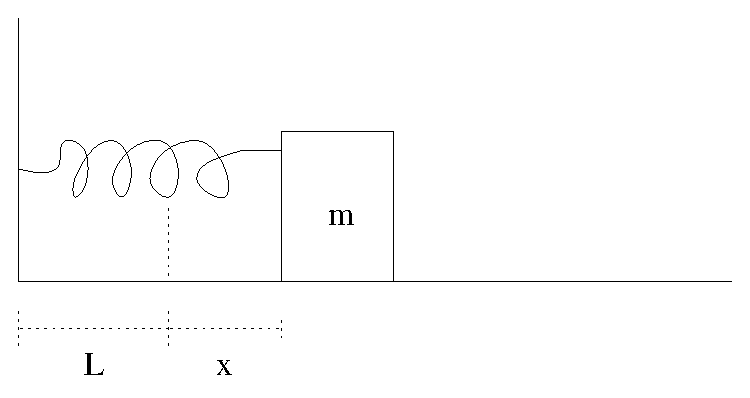
\psfig{file=figures/spring.eps,height=1.5in}}
      \caption{Hooke's Law spring.}
      \label{F:spring2}
\end{figure}


\subsection*{A Reduction to a First Order System}
\index{first order!reduction to}

There is a simple trick that reduces a single linear second order
differential equation to a system of two linear first order equations.
For example, consider the linear homogeneous ordinary differential
equation \Ref{eq:soex1}.  To reduce this second order equation to a first order
system, just set $y=\dot{x}$.  Then \Ref{eq:soex1} becomes
\[
\dot{y} + by + ax = 0.
\]
It follows that if $x(t)$ is a solution to \Ref{eq:soex1} and
$y(t)=\dot{x}(t)$, then $(x(t),y(t))$ is a solution to
\begin{equation}  \label{e:soex1sys}
\begin{array}{rcl}
\dot{x} & = & y \\
\dot{y} & = & -ax - by.
\end{array}
\end{equation}
We can rewrite \Ref{e:soex1sys} as
\[
\dot{X} = Q X.
\]
where
\begin{equation}  \label{e:coeffmatQ}
Q =  \mattwo{0}{1}{-a}{-b}.
\end{equation}
Note that if $(x(t),y(t))$ is a solution to \Ref{e:soex1sys}, then
$x(t)$ is a solution to \Ref{eq:soex1}.  Thus solving the single
second order linear equation is exactly the same as solving the
corresponding first order linear system.

\subsubsection*{The Initial Value Problem}
\index{initial value problem!for second order equations}

To solve the homogeneous system \Ref{e:soex1sys} we need to specify
two initial conditions $X(0)=(x(0),y(0))^t$.  It follows that to
solve the single second order equation we need to specify two initial
conditions $x(0)$ and $\dot{x}(0)$; that is, we need to specify
both initial position\index{initial position} and
initial velocity\index{initial velocity}.

\subsection*{The General Solution}

There are two ways in which we can solve
the second order homogeneous equation \Ref{eq:soex1}.  First,
we know how to solve the system \Ref{e:soex1sys} by finding the
eigenvalues and eigenvectors of the coefficient matrix $Q$ in
\Ref{e:coeffmatQ}.  Second, we know from the general theory of
planar systems that solutions will have the form $x(t)=e^{\lambda_0t}$
for some scalar $\lambda_0$.  We need only determine the values of
$\lambda_0$ for which we get solutions to \Ref{eq:soex1}.

We now discuss the second approach.  Suppose that $x(t)=e^{\lambda_0t}$
is a solution to \Ref{eq:soex1}.  Substituting this form of $x(t)$ in
\Ref{eq:soex1} yields the equation
\[
\left(\lambda_0^2 + b\lambda_0 + a\right)e^{\lambda_0t} = 0.
\]
So $x(t)=e^{\lambda_0t}$ is a solution to \Ref{eq:soex1} precisely
when $p_Q(\lambda_0)=0$, where
\begin{equation} \label{E:charQ}
p_Q(\lambda) = \lambda^2 + b\lambda + a
\end{equation}
is the characteristic polynomial of the matrix $Q$ in \Ref{e:coeffmatQ}.

Suppose that $\lambda_1$ and $\lambda_2$ are distinct real roots of $p_Q$.
Then the general solution\index{general solution} to \Ref{eq:soex1} is
\[
x(t) = \alpha_1e^{\lambda_1t} +  \alpha_2e^{\lambda_2t},
\]
where $\alpha_j\in\R$.

\subsubsection*{An Example with Distinct Real Eigenvalues}

For example, solve the initial value problem
\begin{equation} \label{e:ex12}
\ddot{x} + 3\dot{x} + 2x = 0
\end{equation}
with initial conditions $x(0)=0$ and $\dot{x}(0)=-2$.  The characteristic
polynomial is
\[
p_Q(\lambda) = \lambda^2 + 3\lambda + 2 = (\lambda+2)(\lambda+1),
\]
whose roots are $\lambda_1=-1$ and $\lambda_2=-2$.  So the general solution
to \Ref{e:ex12} is
\[
x(t) = \alpha_1e^{-t} + \alpha_2e^{-2t}
\]
To find the precise solution we need to solve
\[
\begin{array}{rclcl}
x(0) & = & \alpha_1 + \alpha_2 & = & 0 \\
\dot{x}(0) & = & -\alpha_1 - 2\alpha_2 & = & -2
\end{array}
\]
So $\alpha_1 = -2$, $\alpha_2=2$, and the solution to the initial value problem
for \Ref{e:ex12} is
\[
x(t) = -2e^{-t} + 2e^{-2t}
\]

\subsubsection*{An Example with Complex Conjugate Eigenvalues}

Consider the differential equation
\begin{equation} \label{E:ex13}
\ddot{x} -2\dot{x} + 5x = 0.
\end{equation}
The roots of the characteristic polynomial associated to \Ref{E:ex13} are
$\lambda_1=1+2i$ and $\lambda_2=1-2i$.  It follows from the discussion in
the previous section that the general solution to \Ref{E:ex13} is
\[
x(t) = \RE\left(\alpha_1 e^{\lambda_1 t} + \alpha_2 e^{\lambda_2t}\right)
\]
where $\alpha_1$ and $\alpha_2$ are complex scalars.  Indeed, we can rewrite
this solution in real form (using Euler's formula) as
\[
x(t) = e^t\left(\beta_1\cos(2t) + \beta_2\sin(2t)\right),
\]
for real scalars $\beta_1$ and $\beta_2$.

In general, if the roots of the characteristic polynomial are
$\sigma\pm i\tau$, then the general solution to the differential equation is:
\[
x(t) = e^{\sigma t}\left(\beta_1\cos(\tau t) + \beta_2\sin(\tau t)\right).
\]

\subsubsection*{An Example with Multiple Eigenvalues}

Note that the coefficient matrix $Q$ of the associated first order system
in \Ref{e:coeffmatQ} is never a multiple of $I_2$.  It follows from the
previous section
that when the roots of the characteristic polynomial are real and equal,
the general solution has the form
\[
x(t) = \alpha_1 e^{\lambda_1t} + \alpha_2te^{\lambda_2t}.
\]

\subsubsection*{Summary}

It follows from this discussion that solutions to second order
homogeneous linear equations are either a linear combination of two
exponentials (real unequal eigenvalues), $\alpha+\beta t$ times one
exponential (real equal eigenvalues), or a time periodic function times
an exponential (complex eigenvalues).

In particular, if the real part
of the complex eigenvalues is zero, then the solution is time periodic.
The frequency of this periodic solution is often called the {\em internal
frequency}\index{frequency!internal}, a point
that is made more clearly in the next example.


\subsection*{Solving the Spring Equation}

Consider the equation for the frictionless spring without
external forcing.  From \Ref{e:springeq} we get  \index{spring equation}
\index{spring!undamped}
\begin{equation} \label{ex:uspring}
m\ddot{x} + \kappa x = 0.
\end{equation}
where $\kappa>0$.  The roots are $\lambda_1=\sqrt{\frac{\kappa}{m}}i$
and $\lambda_2=-\sqrt{\frac{\kappa}{m}}i$.  So the general solution is
\[
x(t) = \alpha\cos(\tau t) + \beta\sin(\tau t),
\]
where $\tau=\sqrt{\frac{\kappa}{m}}$.  Under these assumptions the
motion of the spring is time periodic with period $\frac{2\pi}{\tau}$
or internal frequency $\frac{\tau}{2\pi}$.  In particular, the solution
satisfying initial conditions $x(0)=1$ and $\dot{x}(0)=0$ (the spring is
extended one unit in distance and released with no initial velocity) is
\[
x(t) = \cos(\tau t).
\]
The graph of this function when $\tau=1$ is given on the
left in Figure~\ref{F:springp}.
\begin{figure}[htb]
           \centerline{%
           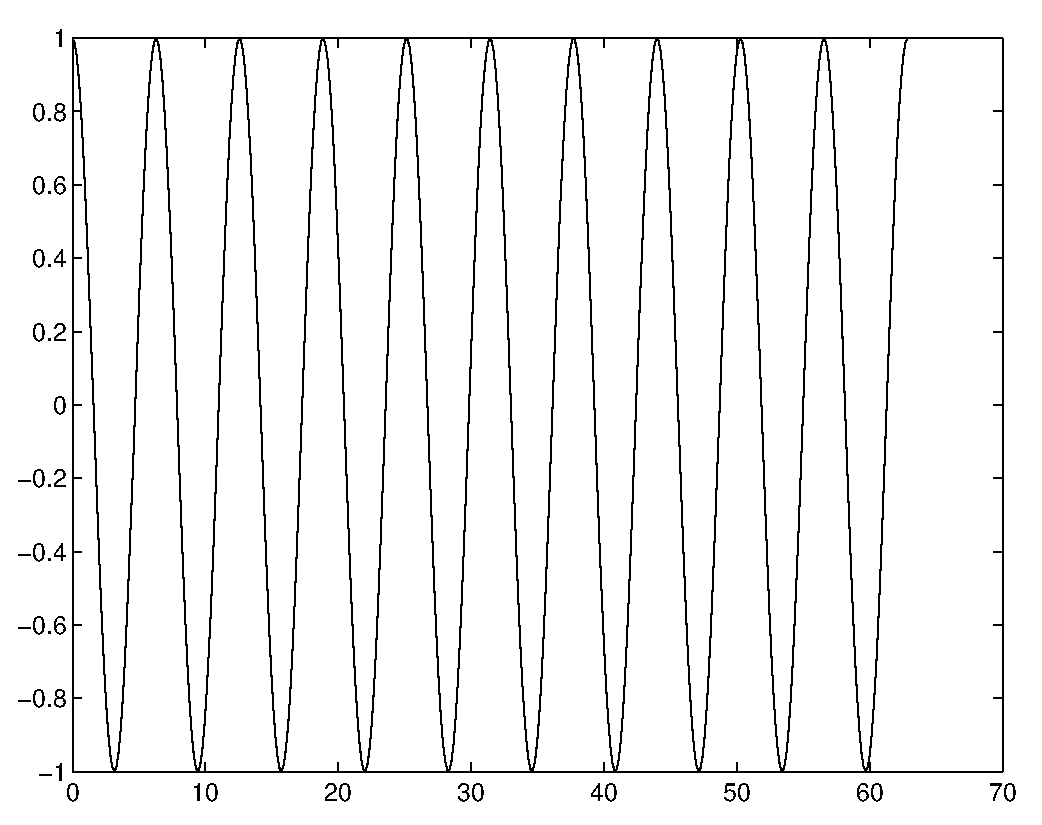
\psfig{file=figures/springp.eps,width=3.0in}
           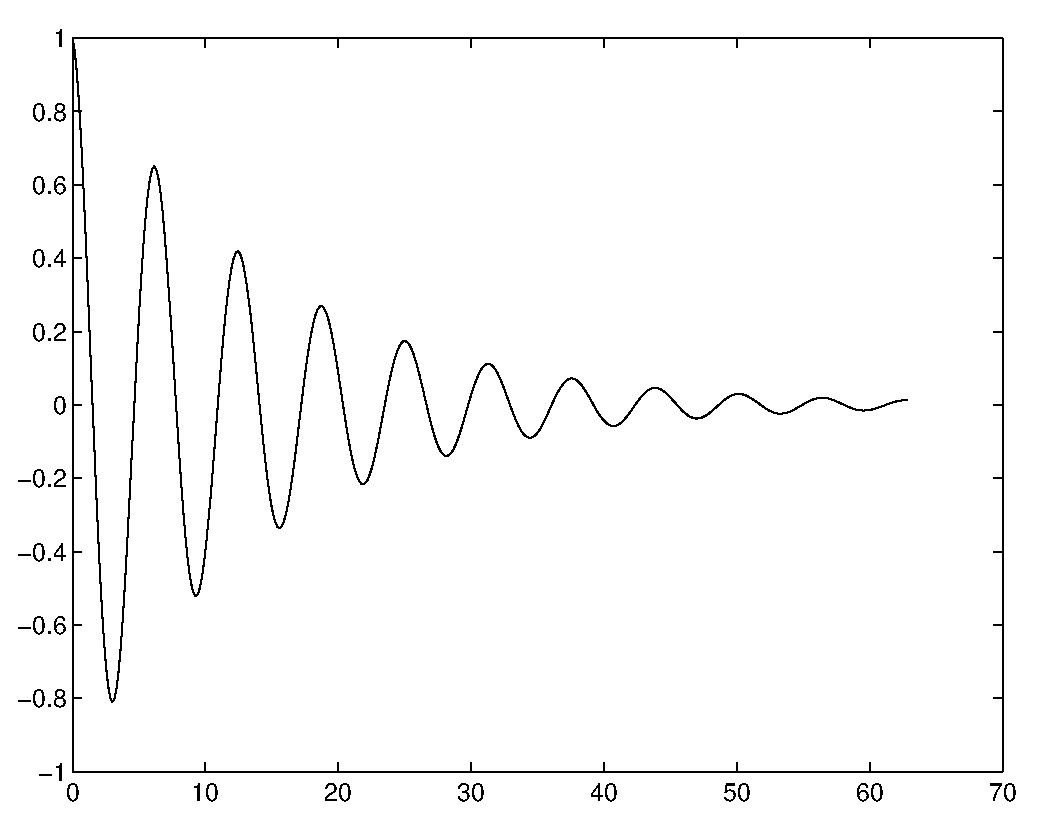
\psfig{file=figures/springpd.eps,width=3.0in}}
           \caption{(Left) Graph of solution to undamped spring
	equation with initial conditions $x(0)=1$ and $\dot{x}(0)=0$.
	(Right) Graph of solution to damped spring equation with the
	same initial conditions.}
           \label{F:springp}
\end{figure}

If a small amount of friction is added, then the spring equation is
\index{spring!damped}
\[
m\ddot{x} + \mu \dot{x} +\kappa x = 0
\]
where $\mu>0$ is small.  Since the eigenvalues of the characteristic
polynomial are $\lambda=\sigma\pm i\tau$ where
\[
\sigma = -\frac{\mu}{2m} < 0 \AND \tau =\sqrt{\frac{\kappa}{m}
-\left(\frac{\mu}{2m}\right)^2},
\]
the general solution is
\[
x(t) = e^{\sigma t}(\alpha\cos(\tau t) + \beta\sin(\tau t)).
\]
Since $\sigma<0$, these solutions oscillate but damp down to zero.  In
particular, the solution satisfying initial conditions $x(0)=1$ and
$\dot{x}(0)=0$ is
\[
x(t) = e^{-\mu t/2m}
\left(\cos(\tau t)-\frac{\mu}{2m\tau}\sin(\tau t)\right).
\]
The graph of this solution when $\tau=1$ and $\frac{\mu}{2m}=0.07$ is
given in Figure~\ref{F:springp} (right).  Compare the solutions for the
undamped and damped springs.

\EXER

\TEXER

\begin{exercise} \label{c6.7.1}
By direct integration solve the differential equation \Ref{e:pointpart}
for a point particle moving only under the influence of gravity.  Find the
solution for a particle starting at a height of $10$ feet above ground with
an upward velocity of $20$ feet/sec.  At what time will the particle hit
the ground?  (Recall that acceleration due to gravity is $32$ feet/sec$^2$.)
\end{exercise}

\begin{exercise} \label{c6.7.2}
By direct integration solve the differential equation \Ref{e:pointpart}
for a point particle moving only under the influence of gravity.  Show
that the solution is
\[
x(t) = -\frac{1}{2}gt^2 + v_0t + x_0
\]
where $x_0$ is the initial position of the particle and $v_0$ is the initial
velocity.
\end{exercise}

\noindent  In Exercises~\ref{c6.6.hoa} -- \ref{c6.6.hoc} find the general
solution to the given differential equation.
\begin{exercise} \label{c6.6.hoa}
$\ddot{x} + 2\dot{x} - 3x = 0$.
\end{exercise}
\begin{exercise} \label{c6.6.hob}
$\ddot{x} - 6\dot{x} + 9x = 0$.
In addition, find the solution to this equation satisfying
initial values $x(1)=1$ and $\dot{x}(1)=0$.
\end{exercise}
\begin{exercise} \label{c6.6.hoc}
$\ddot{x} + 2\dot{x} + 2x = 0$.
\end{exercise}

\begin{exercise} \label{c6.7.3}
Prove that a nonzero solution to a second order linear differential equation
with constant coefficients cannot be identically equal to zero on a nonempty
interval.
\end{exercise}

\begin{exercise} \label{c6.7.4}
Let $r>0$ and $w>0$ be constants, and let $x(t)$ be a solution to the
differential equation
\[
\ddot{x} + r\dot{x} + wx = 0.
\]
Show that $\dps\lim_{t\to\infty} x(t) = 0$.
\end{exercise}

\noindent In Exercises~\ref{c6.6.tfa} -- \ref{c6.6.tfc}, let $x(t)$ be a
solution to the second order linear homogeneous differential equation
\Ref{eq:soex1}.  Determine whether the given statement is {\em true\/}
or {\em false}.
\begin{exercise} \label{c6.6.tfa}
If $x(t)$ is nonconstant and time periodic, then the
roots of the characteristic polynomial are purely imaginary.
\end{exercise}
\begin{exercise} \label{c6.6.tfb}
If $x(t)$ is constant in $t$, then one of the roots of
the characteristic polynomial is zero.
\end{exercise}
\begin{exercise} \label{c6.6.tfc}
If $x(t)$ is not bounded, then the roots of the characteristic
polynomial are equal.
\end{exercise}

\begin{exercise} \label{c3.5.5}
Consider the second order differential equation
\begin{equation}  \label{E:2ndorder}
\frac{d^2x}{dt^2} + a(x)\frac{dx}{dt} + b(x) = 0.
\end{equation}
Let $y(t)=\dot{x}(t)$ and show that \Ref{E:2ndorder} may be
rewritten as a first order coupled system in $x(t)$ and $y(t)$
as follows:
\begin{eqnarray*}
\dot{x} & = & y \\
\dot{y} & = & -b(x) - a(x) y.
\end{eqnarray*}
\end{exercise}


\CEXER

\begin{exercise} \label{c6.7.5}
Use {\sf pplane5} to compute solutions to the system corresponding to the
spring equations with small sliding friction.  Plot the time series (in $x$)
of the solution and observe the oscillating and damping of the solution.
\end{exercise}







